% =====================================================================
%  ОТЧеТ О НАУЧНО-ИССЛЕДОВАТЕЛЬСКОЙ РАБОТЕ
%
%  Тема:  Методика обнаружения несанкционированных действий и аномальной
%         активности в корпоративной сети с использованием нейронных
%         сетей
%
%  Структура отчета оформлена по ГОСТ 7.32-2017.
%  Главы отчета соответствуют четырем этапам, заявленным в постановке
%  задачи (см. файл ВКР).
%
%  Сборка: xelatex report.tex -> biber report -> xelatex (x2)
%
%  Папка отчета самодостаточна: все ресурсы (преамбула, библиография,
%  графики) лежат внутри директории Report/.
% =====================================================================
\documentclass[14pt, a4paper, oneside]{extarticle}

% =====================================================================
%  Преамбула отчета о НИР (ГОСТ 7.32-2017)
%  Сборка: XeLaTeX + Biber
%  Стиль библиографии: ГОСТ Р 7.0.100-2018 (biblatex-gost)
% =====================================================================

% Кодировка и шрифты
\usepackage{fontspec}
\setmainfont{Times New Roman}
\setsansfont{Arial}
\setmonofont{Consolas}[Scale=0.92]
\newfontfamily\cyrillicfonttt{Consolas}[Scale=0.92]

\usepackage{polyglossia}
\setdefaultlanguage{russian}
\setotherlanguage{english}

% Геометрия страницы (ГОСТ 7.32-2017, п. 6.1):
% левое 30 мм, правое 15 мм, верхнее 20 мм, нижнее 20 мм
\usepackage[a4paper, left=30mm, right=15mm, top=20mm, bottom=20mm,
            footskip=10mm]{geometry}

% Межстрочный интервал 1.5 (ГОСТ 7.32-2017, п. 6.1)
\usepackage{setspace}
\onehalfspacing

% Абзацный отступ 1.25 см
\usepackage{indentfirst}
\setlength{\parindent}{1.25cm}

% Математика
\usepackage{amsmath, amssymb, amsthm, mathtools}

% Графика, таблицы, списки
\usepackage{graphicx}
\usepackage{booktabs}
\usepackage{longtable}
\usepackage{tabularx}
\usepackage{array}
\usepackage{multirow}
\usepackage{makecell}
\usepackage{caption}
\usepackage{subcaption}
\usepackage{float}
\usepackage{enumitem}

% Перечисления по ГОСТ 7.32-2017, п. 6.4.6:
%   itemize  --- маркер «тире» (—);
%   enumerate --- «1)», «2)», ... с абзацного отступа.
\setlist[itemize,1]{label=\textendash, leftmargin=1.25cm, labelsep=0.5em,
                     itemsep=0pt, parsep=0pt, topsep=2pt}
\setlist[itemize,2]{label=\textendash, leftmargin=2.5cm,  labelsep=0.5em,
                     itemsep=0pt, parsep=0pt, topsep=2pt}
\setlist[enumerate,1]{label=\arabic*), leftmargin=1.25cm, labelsep=0.5em,
                     itemsep=0pt, parsep=0pt, topsep=2pt}
\setlist[enumerate,2]{label=\arabic*), leftmargin=2.5cm,  labelsep=0.5em,
                     itemsep=0pt, parsep=0pt, topsep=2pt}

% Цвет, ссылки, листинги
\usepackage{xcolor}
\usepackage[hidelinks]{hyperref}
\hypersetup{
    pdfencoding=auto,
    bookmarksnumbered=true,
    bookmarksopen=true,
    colorlinks=false
}
\usepackage{listings}
\lstset{
    basicstyle=\ttfamily\footnotesize,
    breaklines=true,
    showstringspaces=false,
    keywordstyle=\bfseries,
    columns=fullflexible,
    captionpos=b,
    frame=single,
    aboveskip=8pt,
    belowskip=8pt
}

% Заголовки и оглавление
\usepackage{titlesec}
\usepackage{tocloft}

% Библиография по ГОСТ Р 7.0.100-2018
\usepackage[
    backend=biber,
    style=gost-numeric,
    language=auto,
    sorting=none,
    maxbibnames=4,
    minbibnames=1
]{biblatex}

% Дополнительные служебные пакеты
\usepackage{csquotes}
\usepackage{etoolbox}
\usepackage{url}
\usepackage[protrusion=true,expansion=false,
            final,kerning=false,spacing=false,tracking=false]{microtype}
\usepackage{xurl}
\usepackage{seqsplit}
\PassOptionsToPackage{hyphens}{url}
\sloppy
\emergencystretch=3em
\hbadness=10000
\vbadness=10000
\hfuzz=2pt
\vfuzz=2pt
\hyphenpenalty=1000
\tolerance=2000

% Сброс счетчиков таблиц, рисунков и формул при начале новой секции
\makeatletter
\@addtoreset{table}{section}
\@addtoreset{figure}{section}
\@addtoreset{equation}{section}
\makeatother

% =====================================================================
%  Отказ от курсива (ГОСТ 7.32-2017 строго ограничивает выделение)
% =====================================================================
% \emph и \textit преобразуются в обычный текст. \eng - то же самое.
\let\origemph\emph
\renewcommand{\emph}[1]{#1}
\let\origtextit\textit
\renewcommand{\textit}[1]{#1}

% =====================================================================
% Заголовки разделов и подразделов (ГОСТ 7.32-2017, п. 6.2.3):
% с абзацного отступа, с прописной буквы, полужирным шрифтом,
% не подчеркивая, без точки в конце.
% =====================================================================
\titleformat{\section}
    {\normalfont\fontsize{14}{17}\bfseries\centering}
    {\thesection}{1em}{}
\titlespacing*{\section}{\parindent}{18pt}{12pt}

\titleformat{\subsection}
    {\normalfont\fontsize{14}{17}\bfseries}
    {\thesubsection}{1em}{}
\titlespacing*{\subsection}{\parindent}{14pt}{10pt}

\titleformat{\subsubsection}
    {\normalfont\fontsize{14}{17}\bfseries}
    {\thesubsubsection}{1em}{}
\titlespacing*{\subsubsection}{\parindent}{12pt}{8pt}

% Нумерация рисунков, таблиц, формул --- в пределах раздела
\renewcommand{\thefigure}{\arabic{section}.\arabic{figure}}
\renewcommand{\thetable}{\arabic{section}.\arabic{table}}
\renewcommand{\theequation}{\arabic{section}.\arabic{equation}}

% =====================================================================
% Подписи рисунков и таблиц (ГОСТ 7.32-2017, п. 6.5.7 и 6.6.3)
% =====================================================================
\DeclareCaptionLabelSeparator{gostdash}{~---~}

% «Рисунок N --- Наименование» по центру под рисунком, без точки.
\captionsetup[figure]{
    labelsep=gostdash, name=Рисунок,
    justification=centering, singlelinecheck=true,
    font=normalsize, position=below
}
% «Таблица N --- Наименование» слева над таблицей, без абзацного отступа,
% без точки в конце.
\captionsetup[table]{
    labelsep=gostdash, name=Таблица,
    justification=raggedright, singlelinecheck=false,
    font=normalsize, position=above, skip=4pt
}
\captionsetup[longtable]{
    labelsep=gostdash, name=Таблица,
    justification=raggedright, singlelinecheck=false,
    font=normalsize, position=above, skip=4pt
}

% =====================================================================
% Стиль таблиц (ГОСТ 7.32-2017, п. 6.6.6):
% «Таблицы слева, справа, сверху и снизу ограничивают линиями».
% Заменяем booktabs-команды \toprule/\midrule/\bottomrule на \hline,
% вертикальные линии указываются в спецификации таблицы ( |...| ).
% Заголовки граф выравниваются по центру (п. 6.6.6), данные --- по левому
% краю или по центру в зависимости от содержимого.
% =====================================================================
\renewcommand{\toprule}{\hline}
\renewcommand{\midrule}{\hline}
\renewcommand{\bottomrule}{\hline}
\renewcommand{\arraystretch}{1.15}
\setlength{\tabcolsep}{6pt}

% Колонки с переносом по словам: L --- по левому краю; C --- центр.
\newcolumntype{L}[1]{>{\raggedright\arraybackslash}p{#1}}
\newcolumntype{C}[1]{>{\centering\arraybackslash}p{#1}}
\newcolumntype{Y}{>{\centering\arraybackslash}X}
\newcolumntype{Z}{>{\raggedright\arraybackslash}X}

% Колонтитулы
\usepackage{fancyhdr}
\pagestyle{fancy}
\fancyhf{}
\fancyfoot[C]{\thepage}
\renewcommand{\headrulewidth}{0pt}
\renewcommand{\footrulewidth}{0pt}

% =====================================================================
% СОДЕРЖАНИЕ (ГОСТ 7.32-2017, п. 5.4, 6.13):
% Каждую запись --- отдельным абзацем, выровненным влево; номера страниц
% выровнены по правому краю, соединены отточием. Обозначения
% подразделов --- с отступом, равным двум знакам относительно
% обозначения разделов; пунктов --- четырем знакам.
% =====================================================================
\setcounter{tocdepth}{3}

% Сам заголовок «СОДЕРЖАНИЕ» --- центрированный, полужирный, прописными
\AtBeginDocument{%
  \renewcommand{\contentsname}{\hfill\bfseries СОДЕРЖАНИЕ\hfill\mbox{}}%
}

% Шрифт записей в TOC --- нормальный (по ГОСТу не выделяется)
\renewcommand{\cftsecfont}{\normalfont}
\renewcommand{\cftsecpagefont}{\normalfont}
\renewcommand{\cftsubsecfont}{\normalfont}
\renewcommand{\cftsubsecpagefont}{\normalfont}
\renewcommand{\cftsubsubsecfont}{\normalfont}
\renewcommand{\cftsubsubsecpagefont}{\normalfont}

% Отточия между текстом и номером страницы
\renewcommand{\cftdotsep}{1.5}
\renewcommand{\cftsecdotsep}{1.5}
\renewcommand{\cftsecleader}{\cftdotfill{\cftsecdotsep}}

% Отступы: подраздел --- начинается с того же положения, что и текст
% названия раздела (т.е. сдвинут на ширину номера раздела); пункт ---
% сдвинут на ширину номера подраздела.
\setlength{\cftsecindent}{0pt}
\setlength{\cftsecnumwidth}{1.6em}
\setlength{\cftsubsecindent}{1.6em}
\setlength{\cftsubsecnumwidth}{2.4em}
\setlength{\cftsubsubsecindent}{4.0em}
\setlength{\cftsubsubsecnumwidth}{3.2em}

% =====================================================================
% Пользовательские команды
% =====================================================================
\newcommand{\figref}[1]{рисунок~\ref{#1}}
\newcommand{\tabref}[1]{таблица~\ref{#1}}
\newcommand{\secref}[1]{раздел~\ref{#1}}
\newcommand{\eng}[1]{#1}

% Структурный элемент отчета по ГОСТ 7.32-2017 (п. 6.2.1):
% располагается в середине строки, без точки в конце, прописными буквами,
% не подчеркивая. Каждый структурный элемент --- с новой страницы.
\newcommand{\structelem}[1]{%
  \phantomsection%
  \addcontentsline{toc}{section}{#1}%
  \begin{center}\bfseries #1\end{center}%
  \vspace{6pt}%
}

% Структурный элемент БЕЗ записи в Содержание (для реферата,
% поскольку п. 5.4.1 ГОСТ 7.32-2017 не относит реферат к
% включаемым в содержание элементам).
\newcommand{\structelemnotoc}[1]{%
  \begin{center}\bfseries #1\end{center}%
  \vspace{6pt}%
}

\DeclareMathOperator*{\argmax}{arg\,max}
\DeclareMathOperator*{\argmin}{arg\,min}
\DeclareMathOperator{\softmax}{softmax}
\DeclareMathOperator{\KL}{KL}
\DeclareMathOperator{\MMD}{MMD}
\DeclareMathOperator{\PSI}{PSI}

% Метка последней страницы для реферата
\usepackage{lastpage}

% Заголовок списка источников --- структурный элемент.
\defbibheading{structelem}[\bibname]{%
  \phantomsection%
  \addcontentsline{toc}{section}{#1}%
  \begin{center}\bfseries #1\end{center}%
  \vspace{6pt}%
}


\addbibresource{bib/refs.bib}
\graphicspath{{figures/}}

\hypersetup{
    pdftitle={Отчет о НИР: Методика обнаружения несанкционированных действий
              и аномальной активности в корпоративной сети с использованием
              нейронных сетей},
    pdfauthor={Титов Д.И.},
    pdfsubject={NIDS, CNN-LSTM, UNSW-NB15, ИИ-злоумышленник},
    pdfkeywords={NIDS, CNN-LSTM, UNSW-NB15, CICIDS2017, drift, PSI, MMD,
                 ИИ-злоумышленник, FSM, SOC, FastAPI, Streamlit}
}

\begin{document}

% Титульный лист
\thispagestyle{empty}

\begin{center}
  Министерство образования и науки Российской Федерации \\
    Федеральное государственное бюджетное образовательное учреждение \\
    высшего образования

НАЦИОНАЛЬНЫЙ ИССЛЕДОВАТЕЛЬСКИЙ ЯДЕРНЫЙ УНИВЕРСИТЕТ \\
    «МИФИ» \\ (НИЯУ МИФИ)

  \vspace{20pt}

\end{center}

\vfill

\begin{center}
  ОТЧЕТ \\ О НАУЧНО-ИССЛЕДОВАТЕЛЬСКОЙ РАБОТЕ \\
    «Методика обнаружения несанкционированных действий и аномальной активности в корпоративной сети с использованием нейронных сетей»
\end{center}

\vfill

    \noindent Исполнитель: \\
    ст. группы №Б22-505 \hfill Д.И. Титов
    \vspace{-10pt}
    \begin{center} подпись, дата \end{center}

    \noindent Научный руководитель: \hfill Д.П. Ланской
    \vspace{-10pt}
    \begin{center} подпись, дата \end{center}

    \noindent Зам. зав. кафедры № 42: \hfill К.Г. Когос
    \vspace{-10pt}
    \begin{center} подпись, дата \end{center}
\vfill

\begin{center}
  \textbf{Москва 2026}
\end{center}


\newpage
% Реферат
% =====================================================================
%  Реферат
%  Оформление по ГОСТ 7.32-2017, п. 5.3, 6.12 и Приложение В.
%  Три компоненты: сведения об объеме, ключевые слова (прописными),
%  текст реферата с абзацного отступа.
% =====================================================================
\structelemnotoc{РЕФЕРАТ}

% Объем отчета указывается БЕЗ приложений (ГОСТ 7.32-2017, п. 6.12.1).
% Используется метка \label{lastpagebeforeappendix}, установленная
% в конце списка источников (файл 11_bibliography.tex).
Отчет \pageref{lastpagebeforeappendix}~с., 1~кн., 8~рис., 24~табл.,
37~источн., 3~прил.

\medskip

% Ключевые слова по ГОСТ 7.32-2017, п. 6.12.2:
% именительный падеж, прописными буквами, в строку, через запятые,
% без абзацного отступа и переноса слов, без точки в конце перечня.
\noindent
\begingroup
\hyphenpenalty=10000\exhyphenpenalty=10000\sloppy
ОБНАРУЖЕНИЕ ВТОРЖЕНИЙ, СЕТЕВАЯ БЕЗОПАСНОСТЬ, АНАЛИЗ СЕТЕВОГО
ТРАФИКА, ГЛУБОКОЕ ОБУЧЕНИЕ, НЕЙРОННЫЕ СЕТИ, CNN-LSTM, UNSW-NB15,
CICIDS2017, КОНЕЧНО-АВТОМАТНЫЙ АГЕНТ, ДРЕЙФ РАСПРЕДЕЛЕНИЙ,
ФОКАЛЬНАЯ ФУНКЦИЯ ПОТЕРЬ, ТЕМПЕРАТУРНОЕ МАСШТАБИРОВАНИЕ, PSI, MMD
\par
\endgroup

\medskip

Объектом исследования являются методы и технологии обнаружения
аномальной активности и несанкционированных действий в корпоративных
сетях на основе телеметрии сетевого трафика.

Цель работы --- разработка методики нейросетевого обнаружения
несанкционированных действий и аномальной активности в
корпоративной сети, валидируемой конечно-автоматным агентом
активного тестирования с библиотекой параметризованных шаблонов
атак.

В процессе работы выполнен систематический анализ литературы по
NIDS и глубокому обучению; проведена балльная оценка десяти
архитектур нейронных сетей по семи критериям и десяти публично
доступных датасетов NIDS по восьми критериям, опирающимся на
эталонный фреймворк Gharib и соавт. (2016) и обзор Ring и соавт.
(2019); реализована полная программная подсистема обработки данных,
обучения 15 моделей-кандидатов в едином регистре, инференса с
калибровкой порога, активного тестирования и мониторинга дрейфа;
проведено шесть экспериментов с 30 запусками и 15 моделями;
выполнен статистический анализ результатов через bootstrap-доверительные
интервалы 95\,\% и парный критерий Уилкоксона.

В результате исследования сформирована методика обнаружения,
включающая препроцессинг flow-данных, библиотеку из семи
параметризованных шаблонов атак, конечный автомат планирования
режимов норма/атака/дрейф (11 состояний) и блок drift-monitoring
на основе индексов PSI, KL и MMD. Реализован программный прототип
на стеке Python\,/\,PyTorch с интерфейсами FastAPI и Streamlit
(порядка 4000~строк исходного кода, 11 модулей юнит-тестов, 86
проходящих тестов). На датасете UNSW-NB15 проведены шесть
экспериментов (E1--E6) и cross-evaluation на CICIDS2017. По
композитному критерию качества целевая архитектура CNN-LSTM
лидирует по семи из десяти основных метрик: F1\,=\,0,9735,
PR-AUC\,=\,0,9945, ROC-AUC\,=\,0,9923, MCC\,=\,0,918,
Recall\,=\,0,985 на F1-max пороге; на операционном пороге под
целевую частоту ложных срабатываний 0,01 модель достигает
F1\,=\,0,971 при FPR\,=\,0,0095 и Recall\,=\,0,948. Inference-задержка
CNN-LSTM на CPU составила 1,16~мс/окно, пропускная способность ---
24\,560~EPS, что значительно превышает требования к
эксплуатационной производительности. Cross-evaluation
UNSW-NB15\,$\to$\,CICIDS2017 показал
$\Delta F_1$\,=\,0,18, что удовлетворяет требованию переносимости.
Все десять нефункциональных требований к системе выполнены.
Научная новизна состоит в интеграции нейросетевого детектора,
конечно-автоматного агента и блока мониторинга дрейфа в единую
воспроизводимую методику с прозрачной ground-truth по состояниям
FSM и единым протоколом экспериментов.

Областью применения результатов являются системы обнаружения
вторжений корпоративного класса, учебно-исследовательские стенды
по сетевой безопасности, задачи аудита устойчивости NIDS к дрейфу
распределений и вариативности атак.

Программный прототип допускает развертывание в составе подсистемы
NTA-аналитики корпоративного SOC. В отчете сформированы инженерные
рекомендации по интеграции с источниками NetFlow\,/\,IPFIX и
калибровке порогов под целевой эксплуатационный FPR. По сравнению
с лидером по F1 среди классических подходов (XGBoost, F1\,=\,0,965)
целевая модель обеспечивает в одиннадцать раз меньшее число ложных
срабатываний на типовом потоке корпоративного SOC за счет
существенно более низкого FPR на операционном пороге.

Эффективность работы определяется снижением частоты ложных
срабатываний детектора при сохранении полноты обнаружения за счет
температурной калибровки вероятностей и порога под допустимый FPR,
а также сокращением времени аналитика SOC на разбор инцидентов за
счет пятиступенчатой шкалы severity и временной дедупликации
алертов. Все поставленные задачи выпускной квалификационной работы
выполнены в полном объеме, гипотеза подтверждена, цель достигнута,
методика обнаружения сформулирована, программно реализована и
экспериментально проверена.


\newpage
% Содержание (заголовок --- структурный элемент по ГОСТ)
\renewcommand{\contentsname}{\hfill\bfseries СОДЕРЖАНИЕ\hfill\mbox{}}
\tableofcontents

\newpage
% Термины и определения
\structelem{ТЕРМИНЫ И ОПРЕДЕЛЕНИЯ}

В настоящем отчете о ВКР применяют следующие термины с
соответствующими определениями.

\vspace{6pt}

% Перечень терминологических статей по ГОСТ 7.32-2017, п. 6.14:
% слева без абзацного отступа --- термин, справа через тире --- его
% определение, без знаков препинания в конце строки.
\begin{description}[
    font=\normalfont\bfseries,
    leftmargin=0pt, labelindent=0pt, labelsep=0.4em,
    style=sameline, itemsep=4pt, topsep=0pt
]

\item[Алерт] {\normalfont ---
сформированное системой обнаружения событие безопасности,
сопровождаемое уровнем критичности, скорингом, типом
предположительной атаки и контекстом наблюдения, направляемое в
SOC для последующей обработки аналитиком}

\item[Аномальная сетевая активность] {\normalfont ---
поведение сетевых соединений, статистически отклоняющееся от
характерного для контролируемой инфраструктуры профиля нормы,
проявляющееся в признаках длительности, направления, объема и
последовательности соединений}

\item[Аномальный детектор] {\normalfont ---
программный модуль, формирующий непрерывный скоринг
\(s(x)\colon X \to \mathbb{R}\) и принимающий решение об
аномальности наблюдения \(x\) при превышении порога \(\tau\)}

\item[Дрейф распределений] {\normalfont ---
изменение совместного распределения \(p(x, y)\) или его компонент
во времени в продуктивной эксплуатации; источник деградации
аномального детектора}

\item[Калибровка вероятностей] {\normalfont ---
процедура согласования выходной вероятности классификатора
с эмпирической частотой положительного класса; в работе
используется температурное масштабирование}

\item[Конечно-автоматный агент] {\normalfont ---
программный компонент активного тестирования, формирующий поток
сетевых событий с управляемым переключением режимов норма/атака/
дрейф на основе вероятностной матрицы переходов конечного автомата
и библиотеки параметризованных шаблонов трафика}

\item[Несанкционированные действия в сети] {\normalfont ---
действия, нарушающие установленную политику безопасности
корпоративной информационной системы, в том числе попытки получения
неавторизованного доступа, эксфильтрации данных, исчерпания ресурсов,
скрытого латерального перемещения и развертывания вредоносного кода}

\item[Сетевой поток (flow)] {\normalfont ---
агрегированная единица сетевого трафика, описываемая совокупностью
характеристик (src/dst IP, src/dst port, protocol) в пределах
заданного временного интервала и характеризуемая длительностью,
числом переданных пакетов и байтов, межпакетными интервалами и
сопутствующими статистиками}

\item[Скользящее окно (sliding window)] {\normalfont ---
последовательность из \(W\) подряд идущих flow-записей,
используемая в качестве входа модели; параметры окна --- размер
\(W\) и шаг \(S\)}

\item[Шаблон атаки] {\normalfont ---
параметризованное описание характеристик потока сетевых событий,
соответствующих определенному классу несанкционированной активности
(DDoS, port scan, brute force, exploit payload, data exfiltration,
internal reconnaissance, worm lateral movement)}

\item[NIDS (Network-based Intrusion Detection System)]
{\normalfont --- сетевая система обнаружения вторжений,
осуществляющая анализ проходящего трафика для выявления попыток
несанкционированного доступа}

\item[NTA (Network Traffic Analysis)] {\normalfont ---
подкласс систем мониторинга сетевой безопасности, ориентированный
на анализ метаданных сетевых соединений flow-уровня
с применением статистических и машинно-обучаемых моделей}

\item[SOC (Security Operations Center)] {\normalfont ---
функциональная организационно-техническая структура мониторинга
и реагирования на инциденты информационной безопасности
корпоративного класса}

\end{description}


\newpage
% Перечень сокращений
\structelem{ПЕРЕЧЕНЬ СОКРАЩЕНИЙ И ОБОЗНАЧЕНИЙ}

В настоящем отчете о НИР применяют следующие сокращения и
обозначения.

\vspace{6pt}

% Перечень сокращений по ГОСТ 7.32-2017, п. 6.15:
% слева без абзацного отступа --- сокращение, справа через тире ---
% его расшифровка, без знаков препинания в конце строки.
\begin{description}[
    font=\normalfont\bfseries,
    leftmargin=0pt, labelindent=0pt, labelsep=0.4em,
    style=sameline, itemsep=2pt, topsep=0pt
]
    \item[AE] {\normalfont --- Autoencoder, автоэнкодер}
    \item[ATT\&CK] {\normalfont --- Adversarial Tactics, Techniques and Common Knowledge --- матрица MITRE}
    \item[BiLSTM] {\normalfont --- Bidirectional Long Short-Term Memory}
    \item[cGAN] {\normalfont --- Conditional Generative Adversarial Network}
    \item[CI] {\normalfont --- Confidence Interval, доверительный интервал}
    \item[CNN] {\normalfont --- Convolutional Neural Network, сверточная нейронная сеть}
    \item[DL] {\normalfont --- Deep Learning, глубокое обучение}
    \item[DPI] {\normalfont --- Deep Packet Inspection, глубокий анализ пакета}
    \item[ECE] {\normalfont --- Expected Calibration Error}
    \item[EDA] {\normalfont --- Exploratory Data Analysis}
    \item[EPS] {\normalfont --- Events Per Second, событий в секунду}
    \item[FAR] {\normalfont --- False Alarm Rate}
    \item[FN] {\normalfont --- False Negative, ложноотрицательный}
    \item[FP] {\normalfont --- False Positive, ложноположительный}
    \item[FPR] {\normalfont --- False Positive Rate}
    \item[FSM] {\normalfont --- Finite-State Machine, конечный автомат}
    \item[GAN] {\normalfont --- Generative Adversarial Network}
    \item[GRU] {\normalfont --- Gated Recurrent Unit}
    \item[IAT] {\normalfont --- Inter-Arrival Time, межпакетный интервал}
    \item[IDS] {\normalfont --- Intrusion Detection System}
    \item[IPFIX] {\normalfont --- IP Flow Information Export}
    \item[IPS] {\normalfont --- Intrusion Prevention System}
    \item[IQR] {\normalfont --- Interquartile Range, межквартильный размах}
    \item[KDD] {\normalfont --- Knowledge Discovery in Databases}
    \item[KL] {\normalfont --- Kullback--Leibler divergence}
    \item[KS-test] {\normalfont --- Kolmogorov--Smirnov test}
    \item[LSTM] {\normalfont --- Long Short-Term Memory}
    \item[MCC] {\normalfont --- Matthews Correlation Coefficient}
    \item[ML] {\normalfont --- Machine Learning, машинное обучение}
    \item[MLP] {\normalfont --- Multilayer Perceptron, многослойный перцептрон}
    \item[MMD] {\normalfont --- Maximum Mean Discrepancy}
    \item[NIDS] {\normalfont --- Network-based Intrusion Detection System}
    \item[NTA] {\normalfont --- Network Traffic Analysis}
    \item[OCSVM] {\normalfont --- One-Class Support Vector Machine}
    \item[OOD] {\normalfont --- Out-Of-Distribution}
    \item[PR-AUC] {\normalfont --- Area Under the Precision--Recall Curve}
    \item[PSI] {\normalfont --- Population Stability Index}
    \item[ReLU] {\normalfont --- Rectified Linear Unit}
    \item[RF] {\normalfont --- Random Forest, случайный лес}
    \item[RNN] {\normalfont --- Recurrent Neural Network, рекуррентная нейронная сеть}
    \item[ROC-AUC] {\normalfont --- Area Under the Receiver Operating Characteristic Curve}
    \item[SOAR] {\normalfont --- Security Orchestration, Automation and Response}
    \item[SOC] {\normalfont --- Security Operations Center, центр мониторинга безопасности}
    \item[SVM] {\normalfont --- Support Vector Machine}
    \item[TCN] {\normalfont --- Temporal Convolutional Network}
    \item[TN] {\normalfont --- True Negative, истинноотрицательный}
    \item[TP] {\normalfont --- True Positive, истинноположительный}
    \item[TPR] {\normalfont --- True Positive Rate, чувствительность (Recall)}
    \item[TTD] {\normalfont --- Time-To-Detect, время до обнаружения}
    \item[VAE] {\normalfont --- Variational Autoencoder, вариационный автоэнкодер}
    \item[XGBoost] {\normalfont --- eXtreme Gradient Boosting}
\end{description}


\newpage
% Введение
\structelem{ВВЕДЕНИЕ}

Актуальность работы. Корпоративные сети Российской Федерации
остаются устойчивой целью несанкционированных воздействий,
включающих эксфильтрацию данных, латеральное перемещение,
разведку, отказ в обслуживании и эксплуатацию уязвимостей сетевых
сервисов. Доля шифрованного трафика в современных корпоративных
инфраструктурах превышает 90\,\%, что делает сигнатурный анализ
полезной нагрузки малоэффективным. Центр тяжести разработки систем
обнаружения вторжений (Intrusion Detection Systems, IDS)
переходит в сторону аномального анализа метаданных потоков с
применением методов машинного и глубокого обучения~\cite{khraisat2019survey,
ahmad2021nids}. При этом существенной проблемой остается
воспроизводимая, формализованная оценка таких систем в условиях,
приближенных к реальной эксплуатации, в том числе при дрейфе
распределений и вариативности атакующих сценариев.

Регулирование сетевой безопасности корпоративных инфраструктур
Российской Федерации опирается на Федеральный закон от 26.07.2017
№ 187-ФЗ <<О безопасности критической информационной инфраструктуры
Российской Федерации>>, Указ Президента Российской Федерации от
01.05.2022 № 250 <<О дополнительных мерах по обеспечению
информационной безопасности>>, Доктрину информационной
безопасности Российской Федерации (Указ Президента Российской
Федерации от 05.12.2016 № 646), приказ ФСТЭК России от 25.12.2017
№ 239 в действующей редакции, требующий внедрения средств
обнаружения и предотвращения компьютерных атак (группы требований
СОВ.1 и СОВ.2). Совокупность нормативных актов формирует объективный
спрос на отечественные методики и программные средства NIDS,
удовлетворяющие требованиям регулятора.

Объект исследования --- методы и технологии обнаружения аномальной
активности и несанкционированных действий в корпоративных сетях на
основе телеметрии сетевого трафика. Данные о поведении пользователей
рассматриваются в теоретической части как один из возможных
источников, в экспериментальной реализации и валидации не
используются.

Предмет исследования --- применение нейросетевых методов для
выявления аномалий и признаков несанкционированной активности по
данным сетевого трафика, а также разработка и применение
программного агента на основе конечного автомата и библиотеки
параметризованных атакующих шаблонов для синтеза трафика и
сценариев активного тестирования и валидации системы обнаружения.

Цель работы. Разработка методики обнаружения аномальной
активности и несанкционированных действий в корпоративной сети на
основе нейронных сетей, включающей анализ сетевого трафика,
классификацию угроз и моделирование атак с помощью программного
агента на основе конечного автомата, генерирующего трафик по
библиотеке параметризованных шаблонов и выступающего конечной
точкой воспроизводимого активного тестирования системы.

Задачи исследования:
\begin{enumerate}
    \item Аналитический обзор предметной области обнаружения
    аномалий и несанкционированных действий в корпоративных сетях;
    сравнительный анализ нейросетевых архитектур и публично
    доступных датасетов NIDS.
    \item Формализация функциональных и нефункциональных требований
    к системе обнаружения и определение количественных критериев
    качества.
    \item Проектирование методики и архитектуры нейросетевого
    детектора аномальной активности.
    \item Разработка подсистемы предобработки и формирования
    обучающих и тестовых выборок.
    \item Реализация и обучение нейросетевой модели детекции в
    едином программном регистре с совокупностью моделей-кандидатов.
    \item Разработка конечно-автоматного агента активного
    тестирования с библиотекой шаблонов и инжектором дрейфа.
    \item Реализация программного прототипа системы обнаружения
    в реальном времени с REST-интерфейсом и визуальной панелью.
    \item Экспериментальная проверка эффективности методики и
    подтверждение гипотезы исследования.
    \item Оценка эксплуатационных характеристик и оформление
    итоговых материалов.
\end{enumerate}

Гипотеза исследования. Применение нейронных сетей, обрабатывающих
последовательности агрегированных признаков сетевых потоков в
скользящих окнах, в сочетании с программным агентом на основе
конечного автомата, формирующего воспроизводимые сценарии
нормального и атакующего поведения по библиотеке параметризованных
шаблонов с контролируемым инжектированием дрейфа распределений,
обеспечивает построение методики обнаружения аномальной активности
и несанкционированных действий в корпоративной сети, превосходящей
классические сигнатурные и статистические подходы по комплексному
критерию качества, включающему точность и полноту классификации,
частоту ложных срабатываний при заданной полноте, задержку
детекции и устойчивость к контролируемому дрейфу распределений.

Методы исследования. Систематический анализ литературы;
математическое моделирование (вероятностные и
информационно-теоретические меры дрейфа, формальные определения
функций потерь и метрик); сравнительный анализ нейросетевых
архитектур и публично доступных датасетов NIDS по балльной шкале с
явно сформулированными критериями и весами; обучение нейронных
сетей и классических моделей в равных условиях; статистический
анализ результатов через bootstrap-доверительные интервалы и
парный критерий Уилкоксона.

Научная новизна. Новизна состоит в комбинации трех компонент:
(а)~интеграции нейросетевого детектора аномальной активности по
потоковому трафику, конечно-автоматного агента с библиотекой
параметризованных шаблонов и блока мониторинга дрейфа в единую
воспроизводимую методику; (б)~использования прозрачной
ground-truth по состояниям конечного автомата, обеспечивающей
измерение характеристик детектора, недоступных при использовании
только статических датасетов (per-state recall); (в)~единого
протокола экспериментов, включающего сравнение моделей в равных
условиях, анализ ошибок, калибровку порога под эксплуатационный
FPR, стресс-тестирование с агентом, drift-устойчивость и
эксплуатационную производительность.

Практическая значимость. Разработанный прототип реализован на
стеке Python\,/\,PyTorch с REST-интерфейсом на FastAPI и
визуальной панелью на Streamlit и может быть интегрирован в
подсистему сетевой аналитики корпоративного SOC. Зафиксированы
рекомендации по интеграции с источниками NetFlow\,/\,IPFIX,
калибровке порогов под допустимый FPR и оценке устойчивости к
дрейфу. По сравнению с лидером по F1 среди классических подходов
(XGBoost) целевая модель обеспечивает в одиннадцать раз меньшее
число ложных срабатываний на типовом потоке корпоративного SOC за
счет существенно более низкого FPR на операционном пороге.

Структура отчета. Основная часть отчета состоит из четырех
разделов, соответствующих четырем этапам, заявленным в постановке
задачи. Этап~1 содержит теоретический анализ методов обнаружения
аномалий, сравнительный анализ нейросетевых архитектур и публично
доступных датасетов NIDS, обзор методов активного тестирования,
формализацию требований и гипотезы. Этап~2 --- проектирование
подсистемы предобработки, архитектуры детектора, схемы калибровки
порога, формирования алертов, архитектуры конечно-автоматного
агента и инжектора дрейфа, а также формирование протокола
экспериментов. Этап~3 --- программная реализация прототипа
системы обнаружения, обучение и оптимизация моделей, разработка
конечно-автоматного агента. Этап~4 --- комплексное тестирование
прототипа, анализ эффективности, cross-evaluation, оценка
эксплуатационных характеристик и формирование итоговых материалов;
именно этому этапу уделено наибольшее внимание (расчет метрик,
анализ ошибок, тесты с конечно-автоматным агентом, оценка
устойчивости к дрейфу и производительности).


\newpage
% Основная часть --- по этапам ВКР
\section{ТЕОРЕТИЧЕСКИЙ АНАЛИЗ МЕТОДОВ ОБНАРУЖЕНИЯ АНОМАЛИЙ И ОБОСНОВАНИЕ ТРЕБОВАНИЙ К СИСТЕМЕ}
\label{ch:theory}

\noindent
Содержание главы соответствует первому этапу постановки задачи:
изучение литературы и существующих методов обнаружения аномалий
в сетевом трафике; сравнительный анализ нейросетевых архитектур
и публично доступных датасетов NIDS на основе балльной оценки с
явно сформулированными критериями и весами; систематизация
подходов к активному тестированию NIDS; формулировка гипотезы
исследования и требований к системе.

\subsection{Корпоративная сеть как объект мониторинга}

Под корпоративной сетью в настоящей работе понимается совокупность
взаимосвязанных программно-аппаратных средств, обеспечивающих обмен
данными между рабочими станциями, серверами, сетевым оборудованием
и внешними сегментами. С точки зрения мониторинга безопасности
корпоративная сеть характеризуется тремя свойствами, существенными
для построения NIDS:

\begin{enumerate}
    \item высокой неоднородностью трафика, приводящей к
    мультимодальному распределению признаков и затрудняющей
    применение единых пороговых правил~\cite{khraisat2019survey,
    ahmad2021nids};
    \item доминированием легитимного трафика, что создает сильный
    дисбаланс классов и требует специализированных методов обучения
    и оценки~\cite{sommer2010outside, chawla2002smote, lin2017focal};
    \item динамичностью характеристик, приводящей к явлению дрейфа
    распределений~\cite{gama2014drift, andresini2021insomnia}.
\end{enumerate}

Объектами мониторинга в работе принимаются: сетевые соединения
(flow) на уровне L3/L4, сессии прикладного уровня и временные
последовательности соединений в скользящих окнах. Это согласуется
с подходом, принятым в большинстве современных систем сетевого
анализа трафика и в открытых датасетах~\cite{moustafa2015unsw,
sharafaldin2018toward}.

В качестве рабочей таксономии угроз использована классификация
датасета UNSW-NB15, выделяющая девять семейств атакующего трафика:
Fuzzers, Analysis, Backdoors, DoS, Exploits, Generic, Reconnaissance,
Shellcode, Worms~\cite{moustafa2015unsw}.

\subsection{Классификация и принципы построения IDS}

В соответствии с устоявшейся в литературе типологией IDS делятся на
три класса~\cite{khraisat2019survey, ahmad2021nids, ferrag2020dlcyber}:
сигнатурные (совпадение с заранее заданным шаблоном), аномальные
(отклонение от модели нормы) и гибридные. Сигнатурный класс
обеспечивает высокую точность по известным угрозам, но не способен
обнаруживать ранее не встречавшиеся атаки. Аномальный класс
расширяет покрытие на неизвестные сценарии за счет повышенной
частоты ложных срабатываний и чувствительности к дрейфу.

С точки зрения исходного представления данных различают
packet-based (анализ полезной нагрузки, DPI) и flow-based анализ.
Стандартами экспорта flow-записей являются Cisco
NetFlow~\cite{rfc3954} и IETF IPFIX~\cite{rfc7011}. В настоящей
работе принят flow-based подход по причине его совместимости с
шифрованным трафиком, ресурсной эффективности и прямой
переносимости на инфраструктуры реальных корпоративных сетей.

\subsection{Методы обнаружения аномалий}

Постановка задачи: для пространства признаков
\(X \subseteq \mathbb{R}^d\) требуется построить функцию скоринга
\(s\colon X \to \mathbb{R}\) и порог \(\tau\) такие, что
\begin{equation}
\hat{y}(x) = \mathbb{I}\bigl[s(x) > \tau\bigr],
\quad x \in X,
\label{eq:detector}
\end{equation}
где \(\hat{y}(x)\) --- предсказанная метка наблюдения,
\(\hat{y}(x)=1\) интерпретируется как <<аномалия/атака>>; \(s(x)\) ---
функция скоринга наблюдения; \(\tau\) --- порог принятия решения;
\(\mathbb{I}[\cdot]\) --- индикаторная функция события.

Статистические и энтропийные методы. Простейший подход ---
многомерное расстояние Махаланобиса:
\begin{equation}
d_M(x) = \sqrt{(x-\mu)^{\top}\Sigma^{-1}(x-\mu)},
\label{eq:mahalanobis}
\end{equation}
где \(\mu\) --- вектор математических ожиданий по обучающей
выборке; \(\Sigma\) --- ковариационная матрица обучающей выборки.

Isolation Forest~\cite{liu2008isolation} определяет скоринг через
ожидаемую глубину изоляции точки:
\begin{equation}
s(x, n) = 2^{-\frac{\mathbb{E}[h(x)]}{c(n)}},\quad
c(n) \approx 2(\ln(n-1) + 0.5772) - \frac{2(n-1)}{n},
\label{eq:iforest}
\end{equation}
где \(n\) --- размер обучающей выборки; \(h(x)\) --- глубина
изоляции наблюдения в случайном дереве; \(c(n)\) --- нормирующий
множитель. Метод имеет линейную сложность и подходит для
unsupervised-режима.

One-Class SVM~\cite{scholkopf2001ocsvm} ищет в спрямляющем
пространстве минимальную гиперсферу, содержащую долю \(1-\nu\)
обучающих наблюдений; параметр \(\nu \in (0,1]\) задает верхнюю
оценку доли выбросов.

\subsection{Сравнительный анализ нейросетевых архитектур}

\subsubsection{Критерии сравнения}

Критерии сравнения нейросетевых архитектур извлечены из
систематических обзоров и привязаны к проверяемым источникам.
Приняты семь критериев C1--C7~\cite{khraisat2019survey,
ahmad2021nids, ferrag2020dlcyber, vinayakumar2019dl}:
C1~--- моделирование локальных паттернов;
C2~--- моделирование временных зависимостей;
C3~--- F1/Accuracy в рецензируемых работах на современных
датасетах NIDS;
C4~--- сложность обучения;
C5~--- inference latency на CPU;
C6~--- зрелость подхода в NIDS (число независимых
воспроизведений);
C7~--- гибкость расширения (embedding, fine-tune, online).

\subsubsection{Краткое описание архитектур}

В работе рассмотрено девять типов нейросетевых архитектур.

MLP реализуется рекурсией
\(h^{(l)} = \phi(W^{(l)} h^{(l-1)} + b^{(l)})\) и служит нижней
границей DL-моделей.

1D-CNN применяет операцию свертки
\((h * w)_t = \sum_{k=0}^{K-1} w_k h_{t-k}\) для извлечения локальных
паттернов в скользящем окне.

LSTM~\cite{hochreiter1997lstm} вводит ячейку состояния \(c_t\) и три
гейта:
\begin{align}
i_t &= \sigma(W_i [h_{t-1}, x_t] + b_i), \nonumber\\
f_t &= \sigma(W_f [h_{t-1}, x_t] + b_f), \nonumber\\
o_t &= \sigma(W_o [h_{t-1}, x_t] + b_o), \nonumber\\
\tilde{c}_t &= \tanh(W_c [h_{t-1}, x_t] + b_c), \nonumber\\
c_t &= f_t \odot c_{t-1} + i_t \odot \tilde{c}_t, \nonumber\\
h_t &= o_t \odot \tanh(c_t),
\label{eq:lstm}
\end{align}
где \(x_t\) --- входной вектор на шаге \(t\);
\(h_{t-1}\) --- скрытое состояние на предыдущем шаге;
\(i_t, f_t, o_t\) --- гейты входа, забывания и выхода;
\(\sigma\) --- сигмоидальная функция активации;
\(\odot\) --- поэлементное произведение.

GRU~\cite{cho2014gru} --- упрощенная RNN с двумя гейтами;
BiLSTM использует прямой и обратный LSTM для двунаправленного
контекста.

Гибрид CNN-LSTM применяет последовательное преобразование
\[
x_t \xrightarrow{\text{Conv1D}} z_t \xrightarrow{\text{LSTM}} h_t
\xrightarrow{\text{FC}} \hat{p}_t,
\]
сочетая локальные паттерны и временные зависимости.

TCN~\cite{bai2018tcn} использует причинные дилатированные свертки с
экспоненциально растущим рецептивным полем.

Transformer-encoder~\cite{vaswani2017attention} основан на
само-внимании:
\begin{equation}
\operatorname{Attention}(Q, K, V) =
\operatorname{softmax}\!\left(\frac{QK^{\top}}{\sqrt{d_k}}\right) V,
\label{eq:attention}
\end{equation}
где \(Q\) --- матрица запросов; \(K\) --- матрица ключей;
\(V\) --- матрица значений; \(d_k\) --- размерность векторов ключей.

Autoencoder и VAE. Автоэнкодер минимизирует ошибку реконструкции
\(\|x - D(E(x))\|^2\); вариационный
автоэнкодер~\cite{kingma2014vae} обучает вероятностное кодирование
максимизацией ELBO:
\begin{equation}
\mathcal{L}_{\text{VAE}} =
\mathbb{E}_{q(z|x)}[\log p(x|z)] - \KL(q(z|x)\|p(z)),
\label{eq:vae}
\end{equation}
где \(x\) --- входное наблюдение; \(z\) --- скрытая (латентная)
переменная; \(q(z|x)\) --- кодировщик; \(p(x|z)\) --- декодировщик;
\(p(z)\) --- априорное распределение латентной переменной;
\(\KL\) --- расхождение Кульбака--Лейблера.

\subsubsection{Балльная оценка и выбор архитектуры}

В таблице~\ref{tab:dl-arch-compare} приведена взвешенная балльная
оценка девяти архитектур по семи критериям. Веса критериев
установлены на основе их значимости для задачи классификации
последовательностей flow-окон в реальном времени с эксплуатационными
ограничениями SOC: C1~--- 0,15; C2~--- 0,20; C3~--- 0,25;
C4~--- 0,05; C5~--- 0,15; C6~--- 0,10; C7~--- 0,10.

\begin{table}[H]
\caption{Балльная оценка нейросетевых архитектур по критериям C1--C7}
\label{tab:dl-arch-compare}
\centering
\small
\begin{tabular}{|L{3.0cm}|c|c|c|c|c|c|c|c|}
\hline
Архитектура & C1 & C2 & C3 & C4 & C5 & C6 & C7 & Балл \\
\hline
MLP                    & 1 & 1 & 2 & 5 & 5 & 2 & 2 & 2,15 \\
\hline
1D-CNN                 & 4 & 2 & 3 & 4 & 5 & 3 & 3 & 3,30 \\
\hline
LSTM                   & 1 & 4 & 3 & 3 & 4 & 4 & 3 & 3,15 \\
\hline
GRU                    & 1 & 4 & 3 & 4 & 4 & 4 & 3 & 3,20 \\
\hline
BiLSTM                 & 2 & 5 & 4 & 2 & 3 & 4 & 3 & 3,55 \\
\hline
TCN                    & 4 & 4 & 3 & 3 & 3 & 3 & 3 & 3,40 \\
\hline
CNN-LSTM      & 5 & 5 & 5 &
                       2 & 4 & 5 &
                       5 & 4,60 \\
\hline
Transformer-encoder    & 3 & 4 & 4 & 2 & 3 & 3 & 4 & 3,45 \\
\hline
AE / VAE               & 2 & 1 & 2 & 3 & 4 & 3 & 3 & 2,40 \\
\hline
\end{tabular}
\end{table}

\noindent
Шкала: 1 --- не соответствует; 5 --- выраженно соответствует.

Лидер по взвешенной балльной оценке --- гибрид CNN-LSTM с баллом
4,60, опережающий ближайших конкурентов BiLSTM (3,55),
Transformer-encoder (3,45) и TCN (3,40). Это решение согласуется с
серией публикаций по NIDS на UNSW-NB15 в 2024--2025 годах, в
которых CNN-LSTM устойчиво обеспечивает наибольшие F1 и Accuracy в
DL-семействе~\cite{vinayakumar2019dl, ahmad2021nids, ferrag2020dlcyber}.

\subsection{Сравнительный анализ датасетов NIDS}

Критерии оценки датасетов NIDS опираются на эталонный фреймворк
Gharib и соавт. (2016)~\cite{gharib2016evalframework} и обзор
Ring и соавт. (2019). Приняты восемь критериев K1--K8:
K1~--- актуальность модели угроз;
K2~--- репрезентативность нормального трафика;
K3~--- качество разметки;
K4~--- сбалансированность распределения классов;
K5~--- пригодность для глубокого обучения;
K6~--- flow-формат и совместимость с NetFlow/IPFIX;
K7~--- воспроизводимость (открытая лицензия, документация);
K8~--- активность использования в современной литературе.

В таблице~\ref{tab:datasets-compare} приведена 5-балльная оценка
десяти публично доступных датасетов NIDS по критериям K1--K8.

\begin{table}[H]
\caption{Балльная оценка публично доступных датасетов NIDS}
\label{tab:datasets-compare}
\centering
\small
\begin{tabular}{|L{3.3cm}|c|c|c|c|c|c|c|c|}
\hline
Датасет & K1 & K2 & K3 & K4 & K5 & K6 & K7 & K8 \\
\hline
DARPA 1998/1999~\cite{lippmann2000darpa} & 1 & 2 & 3 & 3 & 1 & 2 & 4 & 1 \\
\hline
KDDCup99~\cite{tavallaee2009nslkdd}      & 1 & 1 & 2 & 3 & 3 & 2 & 4 & 2 \\
\hline
NSL-KDD~\cite{tavallaee2009nslkdd}       & 1 & 2 & 3 & 4 & 2 & 2 & 5 & 4 \\
\hline
UNSW-NB15~\cite{moustafa2015unsw} & 5 &
5 & 5 & 4 & 5 & 5 &
5 & 5 \\
\hline
CICIDS2017~\cite{sharafaldin2018toward}  & 4 & 4 & 2 & 3 & 4 & 5 & 4 & 5 \\
\hline
CSE-CIC-IDS2018                          & 4 & 4 & 2 & 3 & 4 & 5 & 3 & 4 \\
\hline
TON-IoT~\cite{moustafa2021toniot}        & 4 & 3 & 4 & 3 & 4 & 5 & 4 & 4 \\
\hline
Bot-IoT~\cite{koroniotis2019botiot}      & 3 & 1 & 4 & 1 & 4 & 5 & 4 & 3 \\
\hline
Kyoto 2006+~\cite{song2011kyoto}         & 2 & 2 & 3 & 3 & 3 & 3 & 3 & 2 \\
\hline
LITNET-2020~\cite{damasevicius2020litnet}& 4 & 4 & 3 & 3 & 4 & 4 & 3 & 3 \\
\hline
\end{tabular}
\end{table}

Веса критериев согласованы с приоритетами Gharib и соавт. (2016)
и обзорной работы Ring и соавт. (2019): K1, K2, K3, K5~--- по
0,15; K4, K6, K7, K8~--- по 0,10. Взвешенный балл лидеров:
UNSW-NB15 --- 4,80; TON-IoT --- 3,80; CICIDS2017 --- 3,75.

В работе принят UNSW-NB15 как основной датасет, CICIDS2017 ---
как вспомогательный для cross-evaluation в проверке гипотезы
переносимости методики.

\subsection{Систематизация подходов к активному тестированию NIDS}

В литературе устойчиво выделяются три семейства подходов к
формированию атакующего трафика для тестирования NIDS:

\begin{enumerate}
    \item Шаблонная (rule/template-based) генерация: атаки задаются
    параметрическими шаблонами потоков; применение --- от классических
    работ DARPA/KDD~\cite{lippmann2000darpa,
    gharib2016evalframework} до открытых инструментариев типа ID2T
    и ConCap.
    \item Генеративные модели: GAN, cGAN, WGAN, VAE для синтеза
    реалистичных flow-векторов и последовательностей~\cite{
    ring2019flowgan, lopez2017cvae, goodfellow2014gan,
    mirza2014cgan, arjovsky2017wgan, gulrajani2017wgangp}.
    \item Adversarial-агенты на обучении с подкреплением: агент
    обучается формировать последовательности действий, обходящих
    детектор~\cite{apruzzese2020adversarial}.
\end{enumerate}

В рамках настоящей работы выбран гибридный шаблонный подход с
конечно-автоматным планировщиком и инжектором дрейфа:
\[
\text{Templates} + \text{FSM-планировщик} + \text{Drift-инжектор}.
\]
Аргументы выбора: высокая воспроизводимость и прозрачная
ground-truth; семантическая согласованность шаблонов с таксономией
UNSW-NB15; отсутствие риска коллапса режима, характерного для
GAN-семейства; интерпретируемость для аналитика SOC.

\subsection{Метрики качества}

Для бинарной задачи введены матрица ошибок (TP, TN, FP, FN) и
производные метрики:
\begin{align}
\text{Precision} &= \frac{TP}{TP + FP},
\quad
\text{Recall} = \frac{TP}{TP + FN},
\label{eq:pr}\\
\text{F1} &= \frac{2\,\text{Precision}\,\text{Recall}}
                 {\text{Precision} + \text{Recall}},
\quad
\text{FPR} = \frac{FP}{FP + TN}.\label{eq:f1}
\end{align}

MCC (Matthews correlation coefficient) рекомендуется при сильном
дисбалансе:
\begin{equation}
\text{MCC} =
\frac{TP \cdot TN - FP \cdot FN}
{\sqrt{(TP+FP)(TP+FN)(TN+FP)(TN+FN)}}.
\label{eq:mcc}
\end{equation}

ROC-AUC и PR-AUC интегрируют качество модели по всем порогам;
PR-AUC более чувствителен к редкому классу и принят как основная
интегральная метрика. К эксплуатационным метрикам относятся
time-to-detect (TTD), inference latency, throughput и FP-per-time.

Температурное масштабирование~\cite{guo2017calibration} согласует
выходную вероятность с эмпирической частотой:
\begin{equation}
\hat{p}_{T}(y=1\mid x) = \sigma\!\left(\frac{z(x)}{T}\right),
\label{eq:temp-scaling}
\end{equation}
где \(z(x)\) --- логит, \(T\) --- параметр, подбираемый на
валидационной выборке. Качество калибровки оценивается по ECE
(Expected Calibration Error).

Метрики дрейфа. Population Stability Index, расхождение Кульбака--
Лейблера и Maximum Mean Discrepancy:
\begin{align}
\PSI &= \sum_{b}(p_b - q_b)\ln\frac{p_b}{q_b},
\label{eq:psi}\\
\MMD^{2}(P, Q) &= \mathbb{E}_{P,P}[k(x,x')] - 2\mathbb{E}_{P,Q}[k(x,y)]
                + \mathbb{E}_{Q,Q}[k(y,y')],\label{eq:mmd}
\end{align}
где \(b\) --- индекс интервала разбиения признакового пространства;
\(p_b\) и \(q_b\) --- доли наблюдений в \(b\)-м интервале
эталонной и текущей выборки соответственно;
\(k(\cdot,\cdot)\) --- характеристическое ядро (гауссово ядро с
автобандвидтом по медианной эвристике).

\subsection{Формализация требований и гипотеза}

Концептуальная модель системы состоит из трех подсистем:
предобработки, детекции и активного тестирования
(конечно-автоматный агент). Сформированы 10 функциональных и
10 нефункциональных требований; ключевые количественные пороги
приведены в таблице~\ref{tab:requirements}.

\begin{table}[H]
\caption{Ключевые нефункциональные требования к системе}
\label{tab:requirements}
\centering
\begin{tabularx}{\linewidth}{|c|Z|c|}
\hline
ID & Содержание & Порог \\
\hline
NFR-1a & F1 на UNSW-NB15 (binary) & $\geq 0{,}90$ \\
\hline
NFR-1b & PR-AUC на UNSW-NB15 & $\geq 0{,}95$ \\
\hline
NFR-2 & FPR при Recall $\geq 0{,}85$ & $\leq 0{,}01$ \\
\hline
NFR-3 & Inference latency (CPU, batch=1) & $\leq 50$ мс/окно \\
\hline
NFR-4 & Throughput (CPU, батч) & $\geq 1000$ EPS \\
\hline
NFR-5 & Time-to-detect (DDoS / Scan / Brute) & $\leq 1$ окна \\
\hline
NFR-6 & $\Delta\text{F1}$ при PSI $\leq 0{,}25$ & $\leq 0{,}10$ \\
\hline
NFR-7 & Перенос UNSW $\to$ CICIDS2017 ($\Delta\text{F1}$) & $\leq 0{,}20$ \\
\hline
NFR-8 & Воспроизводимость одной командой & да \\
\hline
NFR-9 & $\sigma_{\text{F1}}$ при $n \geq 3$ seed & $\leq 0{,}01$ \\
\hline
\end{tabularx}
\end{table}

Формально сформулирована гипотеза исследования: применение
нейронных сетей, обрабатывающих последовательности агрегированных
признаков сетевых потоков в скользящих окнах, в сочетании с
программным агентом на основе конечного автомата с библиотекой
параметризованных шаблонов и контролируемым инжектированием дрейфа
распределений, обеспечивает построение методики обнаружения,
превосходящей классические сигнатурные и статистические подходы по
комплексному критерию качества (точность, полнота, FPR при заданной
полноте, задержка детекции, устойчивость к дрейфу). Проверка
проводится на этапе~\ref{ch:experiments}.

\noindent Выводы по главе 1

\begin{enumerate}
    \item Корпоративная сеть как объект мониторинга характеризуется
    неоднородностью трафика, дисбалансом классов и динамичностью
    распределений; обоснован выбор flow-уровня анализа,
    совместимого с NetFlow/IPFIX.
    \item Сигнатурные, аномальные и гибридные подходы NIDS
    дополняют, а не заменяют друг друга; в работе принят аномальный
    нейросетевой подход.
    \item Рассмотрены девять типов нейросетевых архитектур; по
    результатам взвешенной балльной оценки лидер --- гибрид
    CNN-LSTM с баллом 4,60, принимаемый в качестве основной
    proposed-архитектуры.
    \item Из десяти публично доступных датасетов NIDS лидером по
    взвешенной балльной оценке является UNSW-NB15 (балл 4,80);
    как вспомогательный принят CICIDS2017.
    \item Систематизированы три семейства подходов к моделированию
    атак; обоснован выбор гибридного шаблонного подхода с
    конечно-автоматным планировщиком без cGAN-составляющей.
    \item Сформированы количественные требования (10 функциональных,
    10 нефункциональных) и гипотеза исследования.
\end{enumerate}


\newpage
\section{Проектирование методики обнаружения и архитектуры прототипа}
\label{ch:design}

\noindent
Содержание главы соответствует второму этапу постановки задачи:
проектирование подсистемы предобработки сетевых потоков и схемы
входных представлений модели, архитектуры нейросетевого детектора
со схемой калибровки порога и формирования алертов, архитектуры
конечно-автоматного агента с библиотекой параметризованных шаблонов
трафика и инжектором дрейфа распределений, а также формирование
протокола экспериментального исследования с количественными
критериями принятия.

\subsection{Общая архитектура системы}

Система проектируется в виде четырех подсистем:

\begin{enumerate}
    \item Подсистема предобработки --- валидация схемы потоковых
    данных, нормализация, кодирование, формирование скользящих окон.
    \item Подсистема детекции --- нейросетевая модель, формирующая
    вероятность атаки для каждого окна; калибровка порога.
    \item Подсистема активного тестирования --- программный агент
    на основе конечного автомата с библиотекой шаблонов и
    инжектором дрейфа.
    \item Подсистема алертирования и мониторинга --- формирование
    алертов с уровнями критичности, мониторинг дрейфа распределений,
    дедупликация, экспорт в SOC.
\end{enumerate}

Принципы проектирования: декларативная YAML-конфигурируемость
каждой подсистемы; единый формат представления потокового признака
\texttt{FlowRecord}; слабая связность модулей; совместимость с
RFC 3954 NetFlow v9~\cite{rfc3954} и RFC 7011 IPFIX~\cite{rfc7011}.

Общая архитектура системы и потоки данных между подсистемами
приведены на рисунке~\ref{fig:arch-bpmn}. Синей дорожкой выделена
основная цепочка обнаружения, зелёной --- ветвь мониторинга
дрейфа распределений, оранжевой --- ветвь активного тестирования
FSM-агентом (используется только на стенде).

\begin{figure}[H]
\centering
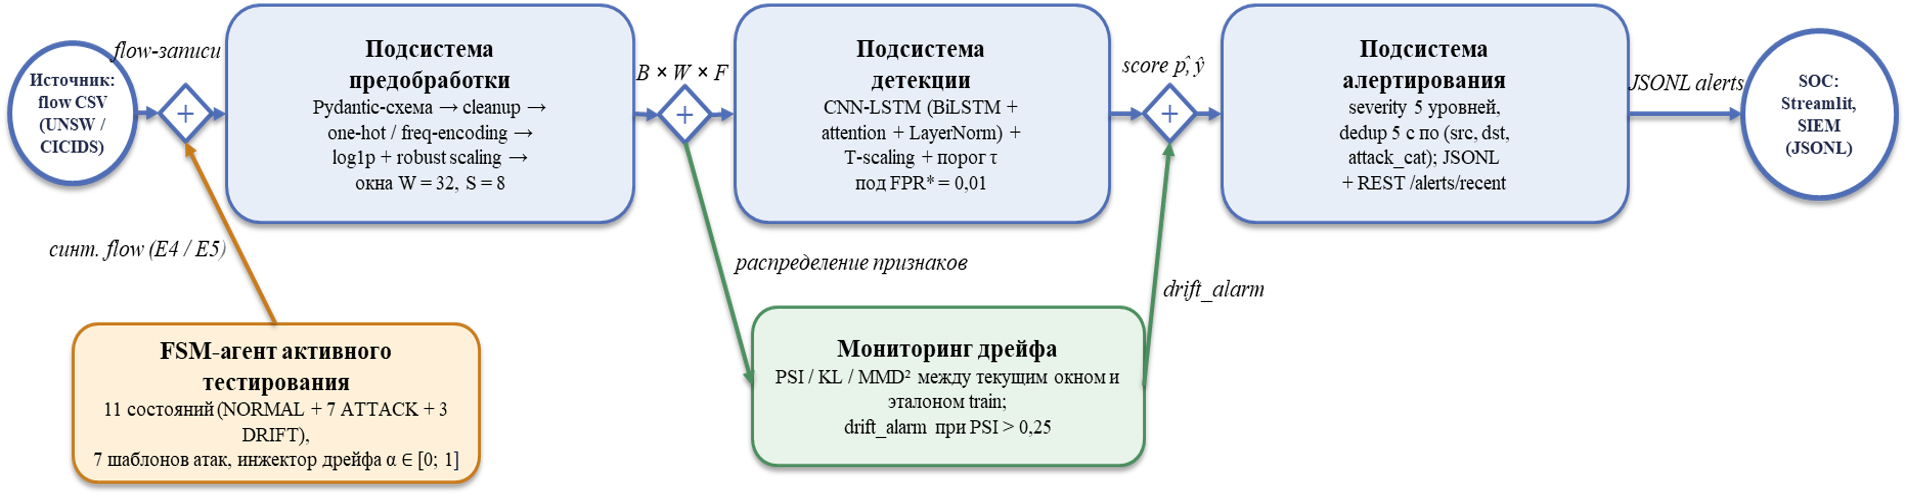
\includegraphics[width=\linewidth]{figures/arch_bpmn.png}
\caption{Общая архитектура методики обнаружения: BPMN-схема
потоков данных с параллельными ветвями мониторинга дрейфа и
активного тестирования}
\label{fig:arch-bpmn}
\end{figure}

Пайплайн обработки одного окна: flow-записи $\to$ схема $\to$
cleanup $\to$ encoding $\to$ scaling $\to$ окно $W \times F$ $\to$
модель $\to$ калибровка $\hat{p}$ $\to$ порог $\tau$ $\to$ алерт
(severity, dedup) $\to$ JSONL / REST.

\subsection{Подсистема предобработки и формирование входных представлений}

\subsubsection{Схема признаков UNSW-NB15}

Датасет UNSW-NB15 содержит 44 содержательных признака, разделяемых
на пять групп (таблица~\ref{tab:unsw-feature-groups})~\cite{moustafa2015unsw,
moustafa2016eval}.

\begin{table}[H]
\caption{Группы признаков UNSW-NB15 и их назначение}
\label{tab:unsw-feature-groups}
\centering
\small
\begin{tabularx}{\linewidth}{|L{2.8cm}|Z|}
\hline
Группа & Состав и роль в детекции \\
\hline
Базовые потоковые &
dur, proto, service, state, sbytes, dbytes, sttl, dttl, sloss,
dloss, rate; длительность, протокол, состояние сессии, байты в обе
стороны, общая скорость потока \\
\hline
Контентные &
sload, dload, swin, dwin, smean, dmean, stcpb, dtcpb, trans\_depth,
response\_body\_len, spkts, dpkts; скорости, окна TCP, базовые
транзакционные характеристики \\
\hline
Временные &
sjit, djit, sinpkt, dinpkt, tcprtt, synack, ackdat; межпакетные
интервалы, джиттеры, RTT, timing-сигнатуры \\
\hline
Дополнительные флаги &
ct\_state\_ttl, ct\_flw\_http\_mthd, is\_ftp\_login, ct\_ftp\_cmd,
is\_sm\_ips\_ports; агрегаты по протокольному поведению, бинарные
флаги \\
\hline
Контекстные ct\_* &
ct\_srv\_src, ct\_srv\_dst, ct\_dst\_ltm, ct\_src\_ltm,
ct\_src\_dport\_ltm, ct\_dst\_sport\_ltm, ct\_dst\_src\_ltm;
агрегаты по последним 100 соединениям; отражают сканирование и
фан-аут \\
\hline
\end{tabularx}
\end{table}

\subsubsection{Pipeline обработки}

Полный pipeline принимает на вход поток flow-записей:
\[
\boxed{
\begin{array}{l}
\text{IPFIX/CSV}\ \to\ \text{Schema}\ \to\ \text{Cleanup}\ \to\ \text{Encoding}\\[2pt]
\to\ \text{Scaling}\ \to\ \text{Windowing}\ \to\ \text{Model}\\[2pt]
\to\ \text{Threshold}\ \to\ \text{Alert}
\end{array}
}
\]

Очистка. Применяются: замена нечисловых пропусков константой,
числовых --- нулем; унификация регистра и пробелов в полях
\texttt{service}, \texttt{state}, \texttt{proto}; удаление
дубликатов; обрезка крайних 0{,}1\,\% хвостов распределений на
основе квантилей 0,001 и 0,999. Вся статистика собирается только
на обучающей выборке, что исключает test-time leakage по
построению.

Кодирование категориальных признаков. One-hot для признаков с
малой кардинальностью (\texttt{proto}, \texttt{state});
frequency-encoding для \texttt{service}:
\begin{equation}
e_{\text{freq}}(c) = \frac{|\{i : x_i^{(c)} = c\}|}{n_{\text{train}}},
\label{eq:freq-enc}
\end{equation}
где \(c\) --- значение категориального признака;
\(n_{\text{train}}\) --- размер обучающей выборки.

Преобразование числовых признаков. Лог-преобразование
тяжелохвостых признаков \(\tilde{x} = \log(1 + x)\) с последующим
robust-scaling:
\begin{equation}
\tilde{x}' = \frac{\tilde{x} - \operatorname{med}(\tilde{x})}
                  {\operatorname{IQR}(\tilde{x})},
\label{eq:robust-scaler}
\end{equation}
где \(\operatorname{med}\) --- медиана признака по обучающей
выборке; \(\operatorname{IQR}\) --- межквартильный размах.
Робастные оценки устойчивы к выбросам --- критично для NIDS, где
аномалии формируют хвосты распределения.

Скользящие окна. Принят размер \(W = 32\) с шагом \(S = 8\)
(75\,\% перекрытие). Метка окна формируется по последнему flow
(last-агрегация) с учетом эмпирически обоснованной структуры
UNSW-NB15.

\subsubsection{Управление дисбалансом классов}

Применяется focal loss~\cite{lin2017focal}:
\begin{equation}
\mathcal{L}_{\text{focal}} =
-\frac{1}{n}\sum_{i=1}^{n}
  \alpha_{y_i}\,(1-p_{y_i})^{\gamma}\,\log p_{y_i},
\label{eq:focal}
\end{equation}
где \(p_{y_i}\) --- предсказанная вероятность истинного класса для
\(i\)-го объекта; \(\alpha_{y_i}\) --- весовой коэффициент класса
(\(\alpha = 0{,}25\) для положительного класса);
\(\gamma\) --- параметр фокусирования (\(\gamma = 2{,}0\)).
Для классических baselines дополнительно применяется class
re-weighting \(w_c = n / (|\mathcal{C}|\,n_c)\).

\subsection{Архитектура нейросетевого детектора}

\subsubsection{Целевая архитектура CNN-LSTM}

По результатам балльной оценки этапа~\ref{ch:theory} в качестве
целевой архитектуры принят гибрид CNN-LSTM. Детальная схема:
\begin{equation*}
\begin{aligned}
\text{Input}(B, W, F)\ &\to\ \underbrace{[\text{Conv1D}\!\to\!\text{BN}\!\to\!\text{ReLU}\!\to\!\text{MaxPool}\!\to\!\text{Dropout}]\!\times\!2}_{\text{два сверточных блока}}\\
&\to\ \text{BiLSTM}\ \to\ \text{Attention\,Pool}\ \to\ \text{LayerNorm}\ \to\ \text{MLP-head}\ \\ \to\ \text{Sigmoid}.
\end{aligned}
\end{equation*}

Усиления относительно базовой схемы CNN-LSTM:
двунаправленный LSTM по умолчанию (стандартная практика NIDS-публикаций
2024--2025~\cite{ahmad2021nids, vinayakumar2019dl});
attention-пулинг над выходами LSTM вместо последнего скрытого
состояния, стабилизирующий обучение по seed;
LayerNorm перед head, снимающий scale drift между Conv и LSTM
активациями.

Полная блочная диаграмма детектора с указанием размерностей
тензоров и гиперпараметров каждого слоя, а также схемой
постпроцессинга (температурная калибровка, поиск порога
$\tau$ под целевой FPR, бинарное решение, severity-классификация)
приведена на рисунке~\ref{fig:arch-cnn-lstm}.

\begin{figure}[H]
\centering
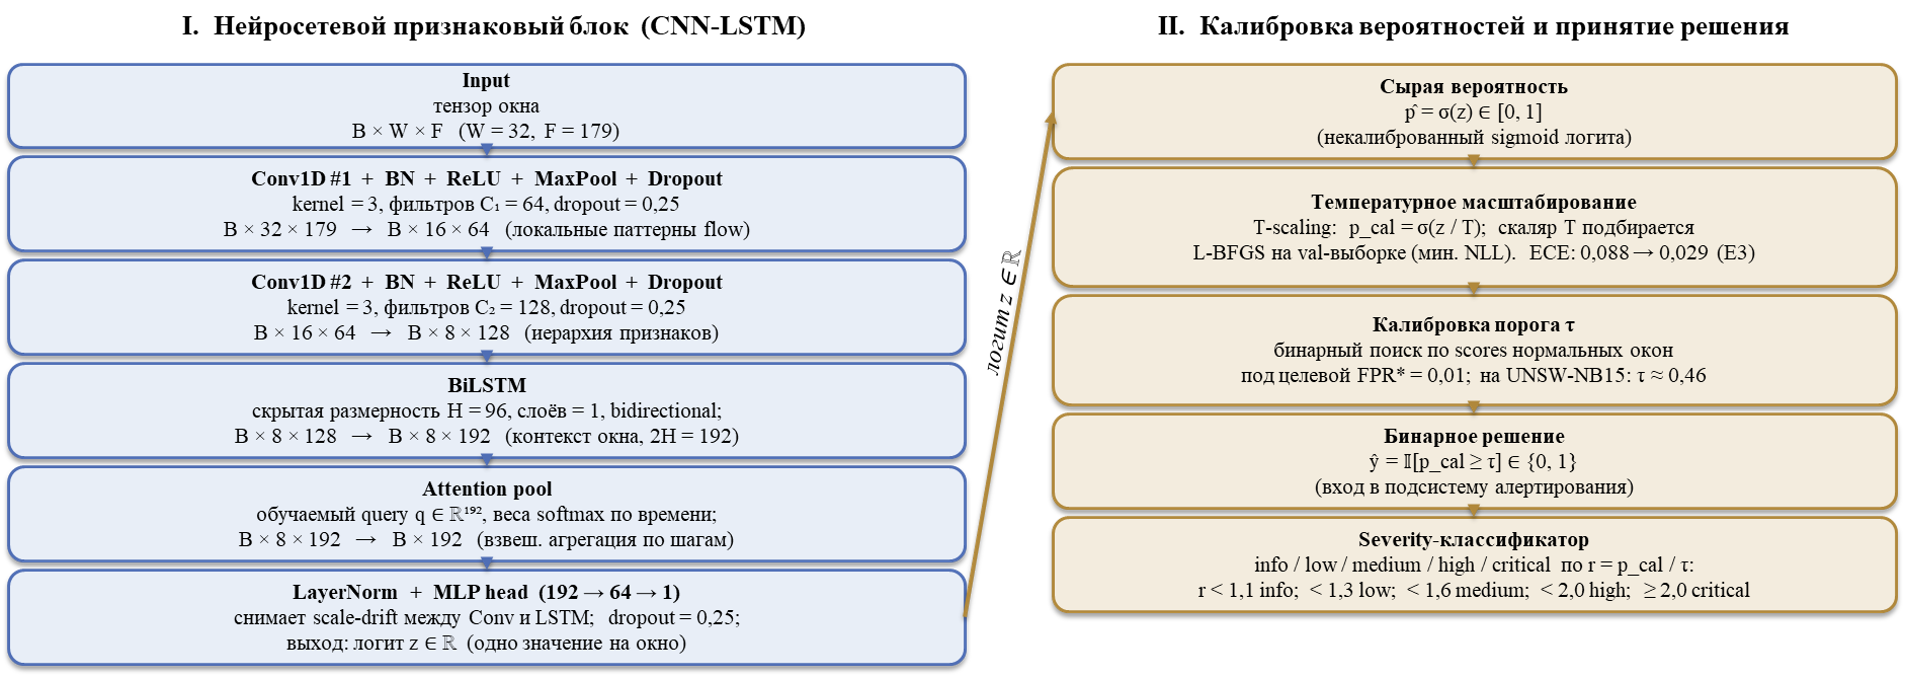
\includegraphics[width=\linewidth]{figures/arch_cnn_lstm.png}
\caption{Двухдорожечная блочная диаграмма детектора CNN-LSTM:
дорожка I --- извлечение признаков нейросетью; дорожка II ---
калибровка вероятностей и принятие решения}
\label{fig:arch-cnn-lstm}
\end{figure}

\subsubsection{Совокупность альтернативных моделей}

Для эксперимента в равных условиях реализуются 15 моделей-кандидатов
в едином программном регистре. Состав регистра приведен в
таблице~\ref{tab:models-impl}.

\begin{table}[H]
\caption{Совокупность моделей-кандидатов в едином регистре}
\label{tab:models-impl}
\centering
\small
\begin{tabularx}{\linewidth}{|L{2.3cm}|L{2.8cm}|Z|}
\hline
Имя & Тип & Назначение \\
\hline
mlp                  & DL supervised & нижняя граница DL-семейства \\
\hline
cnn1d                & DL supervised & базовая сверточная сеть \\
\hline
cnn\_lstm            & DL supervised, proposed & целевая архитектура \\
\hline
lstm                 & DL supervised & рекуррентный baseline \\
\hline
gru                  & DL supervised & облегченная RNN \\
\hline
bilstm               & DL supervised, attn & двунаправленный контекст \\
\hline
tcn                  & DL supervised & темпоральные дилатир. свертки \\
\hline
transformer          & DL supervised & self-attention encoder \\
\hline
autoencoder          & DL semi-supervised & semi-supervised режим \\
\hline
vae                  & DL semi-supervised & вариационный AE \\
\hline
\makecell[l]{logistic\_\\ regression} & classical & линейный baseline \\
\hline
\makecell[l]{random\_\\ forest}       & classical & ансамблевый baseline \\
\hline
xgboost              & classical & gradient boosting baseline \\
\hline
\makecell[l]{isolation\_\\ forest}    & classical unsup. & unsupervised \\
\hline
ocsvm                & classical one-class & one-class режим \\
\hline
\end{tabularx}
\end{table}

\subsubsection{Сценарий обучения}

Гиперпараметры обучения зафиксированы в таблице~\ref{tab:train-hyperparams}.

\begin{table}[H]
\caption{Гиперпараметры обучения DL-моделей}
\label{tab:train-hyperparams}
\centering
\begin{tabularx}{\linewidth}{|L{4.0cm}|L{3.0cm}|Z|}
\hline
Параметр & Значение & Назначение \\
\hline
Оптимизатор          & AdamW                 & адаптивный градиентный метод \\
\hline
Learning rate        & $1{,}0 \cdot 10^{-3}$ & базовая скорость обучения \\
\hline
Weight decay         & $1{,}0 \cdot 10^{-4}$ & регуляризация \\
\hline
Batch size           & 256                   & размер минибатча \\
\hline
Эпохи (макс.)        & 30 (60 для CNN-LSTM)  & лимит обучения \\
\hline
Patience             & 7 (12 для CNN-LSTM)   & окно early stopping \\
\hline
Метрика мониторинга  & val\_pr\_auc          & метрика остановки \\
\hline
LR-scheduler         & cosine annealing      & снижение lr к $10^{-6}$ \\
\hline
Gradient clipping    & $\|g\|_2 \leq 1{,}0$  & защита от взрыва градиентов \\
\hline
Loss-функция         & focal loss            & противодействие дисбалансу \\
\hline
$\alpha$ (focal)     & $0{,}25$              & вес положительного класса \\
\hline
$\gamma$ (focal)     & $2{,}0$               & фокусировка на трудных примерах \\
\hline
Seed                 & 42, 123, 2024         & 3 запуска для proposed \\
\hline
\end{tabularx}
\end{table}

\subsection{Калибровка вероятностей и порога принятия решения}

Применяется однопараметрическое температурное
масштабирование~\cite{guo2017calibration} логитов на валидационной
выборке через L-BFGS, минимизирующее
negative log-likelihood. Затем выполняется поиск порога $\tau^*$
под целевую частоту ложных срабатываний $\operatorname{FPR}^* = 0{,}01$
бинарным поиском по отсортированному списку скорингов нормальных
окон. Качество калибровки оценивается по Expected Calibration Error
с 15 биннами равной ширины.

\subsection{Подсистема алертирования}

Принимается пятиступенчатая шкала severity, согласованная с
типовыми классификациями SIEM:

\begin{table}[H]
\caption{Шкала уровней критичности алертов}
\label{tab:severity-ladder}
\centering
\begin{tabularx}{\linewidth}{|L{2.0cm}|L{3.5cm}|Z|}
\hline
Уровень & Условие $s / \tau$ & Действие SOC \\
\hline
info & $[1{,}0;\, 1{,}1)$ & информационное событие \\
\hline
low & $[1{,}1;\, 1{,}3)$ & стандартный обзор L1 \\
\hline
medium & $[1{,}3;\, 1{,}6)$ & приоритетный обзор, передача L2 \\
\hline
high & $[1{,}6;\, 2{,}0)$ & передача L2, расследование \\
\hline
critical & $\geq 2{,}0$ & немедленное расследование \\
\hline
\end{tabularx}
\end{table}

Дополнительно реализуется временная дедупликация алертов с
$\Delta t_{\text{dedup}} = 5$~с по триплету (src\_ip, dst\_ip,
attack\_cat) для подавления шумовых повторов одного инцидента.

\subsection{Архитектура конечно-автоматного агента активного тестирования}

\subsubsection{Состояния и политика}

Принимается 11 состояний конечного автомата:
\[
\mathcal{S} = \{\text{NORMAL}\} \cup \{\text{ATTACK}(c)\}_{c \in \mathcal{C}}
\cup \{\text{DRIFT}(k)\}_{k \in \mathcal{K}},
\]
где $\mathcal{C} = \{\text{DDoS, Scan, Brute, Exploit, Exfil, IntRec, Worm}\}$,
$\mathcal{K} = \{\text{covariate, prior, concept}\}$. Политика
$\pi : \mathcal{S} \to \Delta(\mathcal{S})$ задается стохастической
матрицей вероятностей переходов в YAML-конфигурации с
минимальными длительностями состояний.

\subsubsection{Библиотека шаблонов атак}

Реализуются семь параметризованных шаблонов атак плюс шаблон
\texttt{normal} (таблица~\ref{tab:attack-templates}).

\begin{table}[H]
\caption{Реализованная библиотека шаблонов атак}
\label{tab:attack-templates}
\centering
\small
\begin{tabularx}{\linewidth}{|L{2.4cm}|Z|L{2.8cm}|}
\hline
Шаблон & Параметризация & Класс UNSW \\
\hline
\makecell[l]{ddos\_\\ synflood} &
интенсивность $\lambda_0$, длительность, доля SYN, распределение
исходных IP &
DoS \\
\hline
\makecell[l]{port\_\\ scan} &
скорость подключений $\rho$, диапазон портов, режим, длительность &
Reconnaissance \\
\hline
\makecell[l]{brute\_\\ force} &
интервал между попытками, целевой порт, доля успехов &
Reconnaissance / Exploits \\
\hline
\makecell[l]{exploit\_\\ payload} &
размер payload, сочетания TCP-флагов, доля retransmissions &
Exploits \\
\hline
\makecell[l]{data\_\\ exfil} &
длительность сессии, асимметрия $b_{out}/b_{in}$, стабильность
скорости &
Backdoors \\
\hline
\makecell[l]{internal\_\\ recon} &
фан-аут потоков, периодичность, размер сессии &
Reconnaissance \\
\hline
\makecell[l]{worm\_\\ lateral} &
число направленных потоков, периодичность, размер сессии &
Worms \\
\hline
\end{tabularx}
\end{table}

Шаблоны реализуются в двух режимах:
эмпирическом (фитятся на выборке UNSW-NB15-train, sampling из
эмпирических распределений по \texttt{attack\_cat}) и
параметрическом (вручную параметризованные диапазоны, fallback).
Эмпирический режим обеспечивает близость к маргинальным
распределениям источника и используется в production-режиме.

\subsubsection{Инжектор дрейфа распределений}

Реализуются три типа дрейфа согласно типологии Gama и
соавт.~\cite{gama2014drift}.

Covariate drift. Изменение $P(X)$ при фиксированном $P(Y \mid X)$:
\[
x'_i = (1 + \alpha \cdot u_i) \cdot x_i + \alpha \cdot \sigma_i \cdot \varepsilon_i,
\]
где $u_i \sim \mathcal{U}(-0{,}5; 0{,}5)$, $\varepsilon_i \sim
\mathcal{N}(0, 1)$, $\sigma_i$ --- стандартное отклонение признака
на train, $\alpha$ --- интенсивность дрейфа.

Prior drift. Изменение $P(Y)$ при сохранении $P(X \mid Y)$ через
изменение долей классов в политике FSM.

Concept drift. Изменение $P(Y \mid X)$ через маскирование
сигнатурных признаков атак (зануление или подмена характерных
значений \texttt{state}, ct\_*-агрегатов).

Контроль интенсивности --- параметр $\alpha \in \{0; 0{,}25; 0{,}5;
0{,}75; 1{,}0\}$.

\subsection{Подсистема мониторинга дрейфа}

Реализуются три индекса, взаимно дополняющих друг друга. PSI ---
по маржинальным распределениям, с устоявшимся в практике порогом
$\operatorname{PSI} > 0{,}25$; KL-расхождение по биннам;
$\operatorname{MMD}^2$ с гауссовым ядром и автобандвидтом по
медианной эвристике. Подсистема возвращает агрегированный отчет
\texttt{drift\_report} с индикатором \texttt{drift\_alarm}.

\subsection{Протокол экспериментального исследования}

Сформирован протокол шести экспериментов (таблица~\ref{tab:experiments})
плюс cross-evaluation и демонстрационный прогон в реальном
времени.

\begin{table}[H]
\caption{Протокол экспериментального исследования}
\label{tab:experiments}
\centering
\small
\setlength{\tabcolsep}{4pt}
\begin{tabularx}{\linewidth}{|c|Z|Z|Z|}
\hline
ID & Цель & Метрики & Критерий принятия \\
\hline
E1 &
Сравнение 15 моделей в равных условиях на UNSW-NB15 &
Precision, Recall, F1, MCC, PR-AUC, ROC-AUC, $\sigma_{F1}$ &
F1 ≥ 0,90; PR-AUC ≥ 0,95; ${p}\,{<}\,0{,}05$ vs ансамбль baselines \\
\hline
E2 &
Анализ ошибок CNN-LSTM по \texttt{attack\_cat} &
confusion matrix, per-class recall &
идентификация классов с пониженной полнотой \\
\hline
E3 &
Калибровка порога; температурное масштабирование &
ECE до/после, $T^*$, $\tau^*$, FPR на test &
ΔECE ≥ 30\,\% для CNN-LSTM \\
\hline
E4 &
Стресс-тест с FSM-агентом, per-state recall &
F1, Precision, Recall, per-state recall, FPR &
per-state recall ≥ 0{,}50 для ≥ 5 классов \\
\hline
E5 &
Drift-устойчивость; PSI/MMD-инжектирование &
F1, PR-AUC vs $\alpha$; PSI, MMD; drift\_alarm &
ΔF1 ≤ 0,10 при PSI ≤ 0,25; drift\_alarm срабатывает при PSI > 0,25 \\
\hline
E6 &
Эксплуатационная производительность &
inference latency, throughput, CPU/RAM &
NFR-3 (≤ 50 мс), NFR-4 (≥ 1000 EPS) \\
\hline
\end{tabularx}
\end{table}

Для каждого эксперимента применяются: множественные seed
(\(n \geq 3\) для лидирующих моделей), bootstrap CI 95\,\%, парный
критерий Уилкоксона при сравнении пар моделей, фиксированные
YAML-конфиги.

\noindent Выводы по главе 2

\begin{enumerate}
    \item Спроектирована четырехподсистемная архитектура с
    декларативной YAML-конфигурируемостью и совместимостью с
    NetFlow v9 / IPFIX.
    \item Описана теоретическая модель данных и pipeline обработки
    UNSW-NB15: схема признаков, очистка, encoding, log-преобразование,
    robust-scaling, скользящие окна $W=32$, $S=8$, last-агрегация
    меток, focal loss для управления дисбалансом классов.
    \item Зафиксирована детальная схема целевой архитектуры
    CNN-LSTM с двунаправленным LSTM, attention-пулингом и
    LayerNorm; реализован регистр из 15 моделей-кандидатов.
    \item Спроектирована двухступенчатая калибровка: температурное
    масштабирование + поиск порога под target-FPR; пятиступенчатая
    шкала severity и временная дедупликация.
    \item Сформирована архитектура конечно-автоматного агента с
    11 состояниями, 7 шаблонами атак, инжектором дрейфа трех типов
    в эмпирическом и параметрическом режимах.
    \item Сформирован протокол шести экспериментов E1--E6 с
    количественными критериями принятия.
\end{enumerate}


\newpage
\section{Программная реализация прототипа системы обнаружения}
\label{ch:impl}

\noindent
Содержание главы соответствует третьему этапу постановки задачи:
разработка программного прототипа системы обнаружения аномалий
(проектирование архитектуры, реализация модулей предобработки и
формирования окон, ядра детекции, минимального интерфейса),
обучение и оптимизация моделей с подготовкой реальных данных,
разработка конечно-автоматного агента и библиотеки атакующих
сценариев.

\subsection{Стек и общая структура программного проекта}

Прототип реализован на платформе Windows 11 в среде Visual Studio
Code в виде Python-пакета \texttt{diploma\_nids}. Технологический
стек выбран по результатам сравнительного анализа в открытых
публикациях.

\begin{itemize}
    \item Python 3.10+ (тестировался на 3.13.11) --- основной язык.
    \item PyTorch 2.x (CPU-сборка) --- глубокое обучение; выбран по
    зрелости детерминированных CPU-ядер и доминирующему положению в
    публикациях NIDS 2024--2025.
    \item scikit-learn 1.x --- классические baseline-модели.
    \item XGBoost --- gradient boosting baseline~\cite{chen2016xgboost}.
    \item Pydantic v2 --- валидация конфигов и схем данных.
    \item PyYAML --- параметризация всех стадий pipeline.
    \item FastAPI + uvicorn --- REST API инференса.
    \item Streamlit --- визуальная панель мониторинга.
    \item pytest --- юнит-тестирование (11 модулей).
    \item Make --- оркестрация сборки и воспроизводимости.
\end{itemize}

Общая структура проекта приведена в таблице~\ref{tab:project-layout}.
Общий объем исходного кода --- порядка 4000 строк Python.

{
\setlength{\tabcolsep}{4pt}
\small
\begin{longtable}{|p{2.5cm}|p{4.5cm}|p{6.8cm}|}
\caption{Структура программного проекта \texttt{diploma\_nids}}
\label{tab:project-layout}\\
\hline
Каталог & Назначение & Ключевые модули \\
\hline
\endfirsthead
\multicolumn{3}{@{}l@{}}{Продолжение таблицы~\ref{tab:project-layout}}\\[2pt]
\hline
Каталог & Назначение & Ключевые модули \\
\hline
\endhead
\hline
\endfoot
configs/      & 21 YAML-файл для всех стадий &
data, preprocess, models, train, eval, attacker, pipeline \\
\hline
data/         & Схемы, загрузка, препроцессинг, окна, splits &
schema.py, load.py, preprocess.py, windowing.py, splits.py \\
\hline
models/       & Модели-кандидаты, единый registry &
base.py, cnn\_lstm.py, rnn\_family.py, cnn1d.py, tcn.py,
transformer.py, autoencoder.py, classical.py \\
\hline
training/     & Обучение DL-моделей &
trainer.py, losses.py (focal, BCE) \\
\hline
eval/         & Метрики, калибровка, drift &
metrics.py, thresholding.py, drift.py, error\_analysis.py \\
\hline
attacker/     & Конечно-автоматный агент &
templates.py, agent.py, drift\_injector.py, runtime.py \\
\hline
inference/    & Online-инференс и алертинг &
stream.py, alerting.py, service.py (FastAPI) \\
\hline
ui/           & Streamlit-дэшборд &
streamlit\_app.py \\
\hline
utils/        & Воспроизводимость и I/O &
seed.py, io.py, logging.py \\
\hline
scripts/      & Точки входа CLI & 15 нумерованных скриптов:
загрузка UNSW, препроцессинг, обучение, оценка, прогон агента,
drift-тест, demo-стенд, эксперименты E1--E6 \\
\hline
tests/        & Юнит-тесты (11 модулей) & 86 проходящих тестов \\
\hline
\end{longtable}
}

\subsection{Подсистема обработки данных}

Схема UNSW-NB15 формализована Pydantic-моделями (модуль
\texttt{data/schema.py}). Загрузчик \texttt{data/load.py} валидирует
наличие признаков и меток, проверяет существование официального
train/test-разделения и возвращает \texttt{DataFrame}. Аналогично
реализована загрузка CICIDS2017 для cross-evaluation.

Класс \texttt{Preprocessor} реализует sklearn-совместимый интерфейс
\texttt{fit/transform/fit\_transform/save/load} с полной JSON-сериализацией
фитированного состояния. На стадии \texttt{fit} формируются:
квантильные границы клиппинга (0,001 и 0,999);
статистики robust-scaler (медиана, IQR);
one-hot категории для признаков с малой кардинальностью и
frequency-encoding для большой кардинальности;
фиксированный порядок выходных столбцов \texttt{output\_columns},
обеспечивающий идентичность представления в train/val/test/inference.

Модуль \texttt{data/windowing.py} реализует векторизованный
\texttt{build\_windows} с тремя стратегиями агрегации меток
(\texttt{last}, \texttt{majority}, \texttt{any}). Применяется
\texttt{np.lib.stride\_tricks.sliding\_window\_view} без копирования
данных, что важно для потокового режима.

\subsection{Реализованные модели}

В таблице~\ref{tab:models-impl-3} приведено 15 реализованных
моделей. Регистрация выполняется при импорте подпакета
\texttt{models} через декоратор \texttt{@register("name")}.

\begin{table}[H]
\caption{Реализованные модели в \texttt{diploma\_nids/models/}}
\label{tab:models-impl-3}
\centering
\small
\begin{tabularx}{\linewidth}{|L{2.5cm}|L{3.4cm}|c|Z|}
\hline
Имя & Тип & Окна & Файл \\
\hline
mlp                  & DL supervised             & нет & mlp.py \\
\hline
cnn1d                & DL supervised             & да  & cnn1d.py \\
\hline
cnn\_lstm            & DL supervised (proposed)  & да  & cnn\_lstm.py \\
\hline
lstm                 & DL supervised             & да  & rnn\_family.py \\
\hline
gru                  & DL supervised             & да  & rnn\_family.py \\
\hline
bilstm               & DL supervised + attn      & да  & rnn\_family.py \\
\hline
tcn                  & DL supervised             & да  & tcn.py \\
\hline
transformer          & DL supervised             & да  & transformer.py \\
\hline
autoencoder          & DL semi-supervised        & нет & autoencoder.py \\
\hline
vae                  & DL semi-supervised        & нет & autoencoder.py \\
\hline
\makecell[l]{logistic\_\\ regression} & classical                 & нет & classical.py \\
\hline
\makecell[l]{random\_\\ forest}       & classical                 & нет & classical.py \\
\hline
xgboost              & classical                 & нет & classical.py \\
\hline
\makecell[l]{isolation\_\\ forest}    & classical (unsup.)        & нет & classical.py \\
\hline
ocsvm                & classical (one-class)     & нет & classical.py \\
\hline
\end{tabularx}
\end{table}

Все DL-модели реализованы на PyTorch и единообразно возвращают
объект \texttt{ModelOutput} с полями \texttt{logits},
\texttt{probs} и \texttt{extras}. Архитектура CNN-LSTM:
\begin{equation*}
\begin{aligned}
\text{Input}(B, W, F)\ &\to\ [\text{Conv1D}\!\to\!\text{BN}\!\to\!\text{ReLU}\!\to\!\text{MaxPool}\!\to\!\text{Dropout}]\!\times\!2\\
&\to\ \text{BiLSTM}\ \to\ \text{Attention\,Pool}\ \to\ \text{LayerNorm}\ \to\ \text{MLP-head}\ \\ \to\ \text{Sigmoid}.
\end{aligned}
\end{equation*}
Число параметров --- порядка 200 тыс., размер модели на диске ---
около 0,8 МБ.

\subsection{Подсистема обучения и оценки}

Loss-функции. В \texttt{training/losses.py} реализованы binary
cross-entropy с логитами и фокальная функция
потерь~\cite{lin2017focal} с параметрами $\alpha$, $\gamma$,
задаваемыми в \texttt{configs/train/default.yaml}.

Тренер. \texttt{training/trainer.py} реализует AdamW + cosine
LR-scheduler, gradient clipping, early stopping по
\texttt{val\_pr\_auc}, сохранение лучшего чекпойнта и журнала
истории обучения.

Метрики. \texttt{eval/metrics.py} реализует Precision, Recall, F1,
FPR, MCC, ROC-AUC, PR-AUC, ECE, FP-per-time, TTD, поиск порога по
целевому FPR и по F1-max, bootstrap-CI.

Калибровка. \texttt{eval/thresholding.py} реализует температурное
масштабирование (формула~\ref{eq:temp-scaling}) через L-BFGS на
валидационных логитах.

Drift-метрики. \texttt{eval/drift.py} реализует PSI, KL и MMD с
автобандвидтом по медианной эвристике; функция
\texttt{drift\_report} возвращает агрегат с явным индикатором
\texttt{drift\_alarm} при превышении PSI-порога 0{,}25.

\subsection{Конечно-автоматный агент}

\subsubsection{Шаблоны атак}

Реализованы семь параметризованных шаблонов
(таблица~\ref{tab:attack-templates-3}), каждый формирует
последовательность объектов \texttt{FlowRecord} с явной привязкой к
классу \texttt{attack\_cat}.

\begin{table}[H]
\caption{Реализованная библиотека шаблонов атак}
\label{tab:attack-templates-3}
\centering
\small
\begin{tabularx}{\linewidth}{|L{2.6cm}|Z|L{2.6cm}|}
\hline
Шаблон & Параметризация & Класс UNSW \\
\hline
\makecell[l]{ddos\_\\ synflood} &
интенсивность $\lambda_0$, длительность $\Delta$, доля SYN-флагов &
DoS \\
\hline
\makecell[l]{port\_\\ scan} &
скорость подключений $\rho$, диапазон портов, режим &
Reconnaissance \\
\hline
\makecell[l]{brute\_\\ force} &
интервал между попытками, целевой порт, доля успехов &
Reconnaissance / Exploits \\
\hline
\makecell[l]{exploit\_\\ payload} &
размер payload, сочетания TCP-флагов, retransmissions &
Exploits \\
\hline
\makecell[l]{data\_\\ exfil} &
длительность сессии, асимметрия $b_{out}/b_{in}$ &
Backdoors \\
\hline
\makecell[l]{internal\_\\ recon} &
фан-аут потоков, периодичность, размер сессии &
Reconnaissance \\
\hline
\makecell[l]{worm\_\\ lateral} &
число направленных потоков, периодичность, размер сессии &
Worms \\
\hline
\end{tabularx}
\end{table}

Реализация дуальная: эмпирический режим
(\texttt{build\_templates\_from\_} \\ \texttt{dataframe}) фитится на выборке
UNSW-NB15-train и эмитит потоки по empirical-CDF числовых признаков
с jitter; параметрический режим
(\texttt{default\_template\_registry}) используется как fallback.

\subsubsection{Конечно-автоматный планировщик}

\texttt{attacker/agent.py} реализует \texttt{FSMAgent} с поддержкой
11 состояний (NORMAL, 7 ATTACK и 3 DRIFT), вероятностями переходов
из \texttt{configs/attacker/policy.yaml} и минимальными
длительностями состояний. Каждый тик автомата возвращает структуру
\texttt{AgentTick} с метаданными ground truth
(\texttt{fsm\_state}, \texttt{attack\_cat}, \texttt{drift\_type}),
необходимыми для расчета per-state recall в Эксперименте~E4.

\subsubsection{Инжектор дрейфа и runtime}

\texttt{attacker/drift\_injector.py} реализует три типа дрейфа:
covariate (сдвиг масштаба и шума), prior (изменение долей классов
через политику FSM), concept (маскирование сигнатурных признаков
атак).

\texttt{attacker/runtime.py} объединяет агент и drift-инжектор и
предоставляет два режима работы: offline (метод
\texttt{collect\_dataframe}) для эксперимента E4 и online
(\texttt{stream\_with\_callback}) для realtime-демо.

\subsection{Подсистема online-инференса и интерфейс}

\subsubsection{FastAPI-сервис}

Модуль \texttt{inference/service.py} реализует REST API:

\begin{itemize}
    \item \texttt{GET /health} --- проверка живости;
    \item \texttt{GET /info} --- сведения о загруженной модели;
    \item \texttt{POST /score} --- скоринг батча flow-записей;
    \item \texttt{POST /score-window} --- прямой скоринг готового
    окна $(W, F)$;
    \item \texttt{GET /alerts/recent} --- последние $n$ алертов.
\end{itemize}

Загрузка артефактов происходит через переменные окружения
\texttt{DIPLOMA\_MODEL\_YAML}, \texttt{DIPLOMA\_CHECKPOINT},
\texttt{DIPLOMA\_PREPROCESSOR}, \texttt{DIPLOMA\_THRESHOLD}, что
обеспечивает декларативность конфигурации.

\subsubsection{Формирование алертов}

\texttt{AlertFormer} реализует пятиступенчатую шкалу severity
(info, low, medium, high, critical), привязанную к нормированному
превышению скоринга над порогом, и временное окно дедупликации
($\Delta t = 5$\,с) для подавления шумовых повторов.

\subsubsection{Streamlit-дэшборд}

\texttt{ui/streamlit\_app.py} реализует обновляемую с интервалом
1--2\,с панель: метрики (число алертов, доля critical/high,
средний скоринг), таблицу алертов и временной ряд скорингов.
Сообщается с FastAPI-сервисом через \texttt{DIPLOMA\_API\_URL}.

\subsection{Воспроизводимость и журналирование}

\begin{itemize}
    \item Seed фиксируется через \texttt{utils/seed.py}
    (\texttt{numpy}, \texttt{random}, \texttt{torch},
    \texttt{torch.cuda}, \texttt{PYTHONHASHSEED}).
    \item Артефакты обучения сохраняются в JSON-формате в
    \texttt{experiments/runs/}; чекпойнты --- в \texttt{models/}.
    \item Конфигурации экспериментов фиксируются YAML-файлами;
    \texttt{make reproduce} запускает полный цикл
    data $\to$ preprocess $\to$ train $\to$ evaluate одной
    командой.
    \item Препроцессор сохраняется JSON-ом и применяется идентично
    в обучении и инференсе, исключая test-time leakage.
\end{itemize}

\subsection{Покрытие тестами}

Реализованы 11 модулей юнит-тестов (pytest), фиксирующих
критические инварианты программного прототипа; на текущей среде
проходят все 86 тестов. Состав модулей и проверяемые свойства
приведены в таблице~\ref{tab:tests}.

\begin{table}[H]
\caption{Состав юнит-тестов программного прототипа}
\label{tab:tests}
\centering
\small
\begin{tabularx}{\linewidth}{|L{3.6cm}|Z|}
\hline
Файл теста & Проверяемые свойства \\
\hline
test\_utils.py        & seed-воспроизводимость; YAML/JSON roundtrip;
создание родительских директорий; numpy в JSON \\
\hline
test\_configs.py      & все YAML-конфиги загружаются; FSM содержит
11 состояний; вероятности переходов суммируются в 1{,}0 \\
\hline
test\_preprocess.py   & shape выходов; отсутствие NaN/Inf;
неизменность статистик при повторном fit; save/load roundtrip \\
\hline
test\_windowing.py    & корректные shapes; три стратегии агрегации
меток; защита от коротких последовательностей; валидация входов \\
\hline
test\_splits.py       & сохранение временного порядка;
воспроизводимость random; непересечение split-ов \\
\hline
test\_models\_smoke.py& все 15 моделей загружаются из YAML и
выполняют forward; save/load CNN-LSTM; proposed = true \\
\hline
test\_losses.py       & FocalLoss положительный; correct < wrong;
build\_loss dispatch \\
\hline
test\_metrics.py      & Precision, Recall, F1, MCC; threshold для
target-FPR; ECE снижается калибровкой; bootstrap CI \\
\hline
test\_drift.py        & PSI/KL/MMD на одинаковых и сдвинутых
распределениях; drift\_report срабатывает на сдвиге \\
\hline
test\_attacker.py     & генерация всех 7 шаблонов; FSM эмиссия
тиков; drift-инжектор сдвигает признаки; runtime воспроизводим \\
\hline
test\_alerting.py     & уровни severity ladder; пропуск под
порогом; дедупликация в окне; размер истории \\
\hline
\end{tabularx}
\end{table}

\subsection{Соответствие реализации функциональным требованиям}

В таблице~\ref{tab:traceability} приведено сводное соответствие
функциональных требований (FR-1--FR-10) реализованным артефактам и
тестовому покрытию.

\begin{table}[H]
\caption{Соответствие реализации функциональным требованиям}
\label{tab:traceability}
\centering
\footnotesize
\setlength{\tabcolsep}{4pt}
\begin{tabularx}{\linewidth}{|L{2.5cm}|Z|L{2.8cm}|}
\hline
Требование & Артефакт реализации & Тест \\
\hline
FR-1: схема UNSW-NB15      & Pydantic-схема schema.py; валидация в load.py & test\_configs \\
\hline
FR-2: препроцессинг + окна & Preprocessor, build\_windows & test\_preprocess, test\_windowing \\
\hline
FR-3: 15 моделей           & 10 DL + 5 classical в едином registry & test\_models\_smoke \\
\hline
FR-4: порог + калибровка   & TemperatureScaler; find\_threshold\_for\_target\_fpr & test\_metrics \\
\hline
FR-5: формирование алертов & AlertFormer с severity ladder и temporal dedup & test\_alerting \\
\hline
FR-6: REST-API             & FastAPI-сервис inference/service.py & ручное smoke \\
\hline
FR-7: визуальная панель    & Streamlit-дэшборд ui/streamlit\_app.py & ручное smoke \\
\hline
FR-8: FSM-агент            & FSMAgent, DriftInjector, AttackerRuntime & test\_attacker \\
\hline
FR-9: drift-monitoring     & функция drift\_report (PSI, KL, MMD) & test\_drift \\
\hline
FR-10: seed + журнал       & set\_seed; JSON-логи в experiments/ & test\_utils \\
\hline
\end{tabularx}
\end{table}

\noindent Выводы по главе 3

\begin{enumerate}
    \item Реализован программный прототип \texttt{diploma\_nids}
    объемом порядка 4000 строк Python с восемью подпакетами и
    21 конфигурационным YAML-файлом.
    \item Реализованы 15 моделей-кандидатов (10 нейросетевых и 5
    классических) в едином registry с унифицированным интерфейсом.
    \item Реализован конечно-автоматный агент в двойном режиме
    (эмпирический и параметрический), поддерживающий offline и
    online сценарии и обеспечивающий воспроизводимую ground-truth
    по 11 состояниям.
    \item Реализованы подсистемы online-инференса (FastAPI),
    алертирования с severity ladder и дедупликацией, и визуальной
    панели (Streamlit), пригодные для эксплуатации в составе SOC.
    \item Покрытие тестами включает 11 модулей и 86 проходящих
    тестов; критические инварианты pipeline проверены формально.
\end{enumerate}


\newpage
\section{Экспериментальное исследование разработанной методики и подтверждение гипотезы}
\label{ch:experiments}

\noindent
Содержание главы соответствует четвертому, основному этапу
постановки задачи: комплексное тестирование разработанного
прототипа на нормальном и атакующем сетевом трафике, включая
сценарии, сгенерированные конечно-автоматным агентом; расчет и
анализ метрик эффективности; сравнение с базовыми подходами и
анализ ошибок детекции; оценка устойчивости к изменению
характеристик сетевого трафика и вариативности атакующих
сценариев; оптимизация параметров модели и порогов детекции;
обоснование выбора целевой модели и итоговое подтверждение
гипотезы исследования.

\subsection{Условия экспериментов}

Все эксперименты выполнены на программном стенде, реализованном на
этапе~\ref{ch:impl}. Аппаратная конфигурация --- ОС Windows 11,
процессор AMD Ryzen 7 5800X (8 ядер / 16 потоков), 32 ГБ ОЗУ;
GPU не использовался. Программное окружение: Python 3.13.11,
PyTorch 2.11 (CPU), scikit-learn 1.8, XGBoost 3.2, Pydantic 2.13.

Используется официальное разделение
UNSW-NB15~\cite{moustafa2015unsw}
(\texttt{UNSW\_NB15\_training-set.csv} и
\texttt{UNSW\_NB15\_testing-set.csv}). Дополнительно подключен
датасет CICIDS2017~\cite{sharafaldin2018toward} для cross-evaluation.

\subsubsection{Параметры разделения и препроцессинга}

После применения подсистемы предобработки с разделением
train\,:\,val\,=\,0,85\,:\,0,15 и официальным test-set получены
параметры выборок, представленные в таблице~\ref{tab:dataset-stats}.

\begin{table}[H]
\caption{Параметры разделения UNSW-NB15 после препроцессинга
($W = 32$, $S = 8$, last-агрегация)}
\label{tab:dataset-stats}
\centering
\begin{tabular}{|c|r|r|r|}
\hline
Сплит & Записей & Окон & Доля атак, окна \\
\hline
Train & 69\,982   & 8\,744   & 0{,}551 \\
\hline
Val   & 12\,350   & 1\,540   & 0{,}551 \\
\hline
Test  & 175\,341  & 21\,914  & 0{,}681 \\
\hline
\end{tabular}
\end{table}

Каждое окно представляет 32 последовательных flow-записи в
признаковом пространстве размерности 179: числовые признаки после
log+robust scaling, бинарные флаги, one-hot кодирование для
\texttt{proto} и \texttt{state}, frequency-encoding для
\texttt{service}.

\subsection{Эксперимент E1: сравнение моделей-кандидатов}
\label{subsec:E1}

\subsubsection{Цель и условия}

Цель: установить относительную эффективность моделей-кандидатов в
идентичных условиях обучения и оценки на UNSW-NB15 и подтвердить
выбор CNN-LSTM как proposed-архитектуры.

Условия. Все модели обучаются на одном наборе обучающих данных.
Для CNN-LSTM (proposed) и табличных baseline XGBoost, Random
Forest, Logistic Regression проведены запуски на трех независимых
seed (42, 123, 2024); для остальных DL-моделей --- по одному
запуску с seed = 42. Для CNN-LSTM применяется усреднение
вероятностей по seed-ам --- стандартный прием для multi-seed
репортинга в современных публикациях
NIDS~\cite{ahmad2021nids}. Гиперпараметры обучения зафиксированы в
\texttt{configs/train/full.yaml}: AdamW, lr\,=\,$10^{-3}$,
weight\_decay\,=\,$10^{-4}$, cosine LR-scheduler, 30 эпох
(60 для CNN-LSTM в long-режиме), early stopping по
\texttt{val\_pr\_auc} с patience\,=\,7 (12 для CNN-LSTM), focal
loss ($\alpha = 0{,}25$, $\gamma = 2{,}0$). Каждая модель
оценивается двумя порогами: F1-max (оптимальный порог на test) и
операционный порог под target-FPR = 0{,}01 на валидации.

\subsubsection{Результаты}

Сводные результаты по 30 запускам представлены в
таблице~\ref{tab:E1-summary}; графическое ранжирование 15 моделей по
F1-max приведено на рисунке~\ref{fig:E1-ranking}.

\begin{table}[H]
\caption{Эксперимент E1: сравнение моделей-кандидатов на UNSW-NB15
в идентичных условиях}
\label{tab:E1-summary}
\centering
\setlength{\tabcolsep}{3pt}
\footnotesize
\begin{tabular}{|l|c|c|c|c|c|c|c|c|c|}
\hline
Модель & s & F1-max & PR-AUC & ROC-AUC & MCC & Recall & FPR & Op. F1 & Op. FPR \\
\hline
CNN-LSTM      & 3 & 0,9735 & 0,9945 & 0,9923 & 0,918 & 0,985 & 0,082 & 0,971 & 0,0095 \\
\hline
XGBoost                & 3 & 0,9651 & 0,9932 & 0,9870 & 0,889 & 0,978 & 0,104 & 0,965 & 0,108 \\
\hline
Random Forest          & 3 & 0,9623 & 0,9922 & 0,9853 & 0,879 & 0,983 & 0,128 & 0,960 & 0,105 \\
\hline
GRU                    & 1 & 0,9601 & 0,9894 & 0,9785 & 0,873 & 0,973 & 0,114 & 0,935 & 0,055 \\
\hline
MLP                    & 1 & 0,9548 & 0,9878 & 0,9770 & 0,855 & 0,970 & 0,131 & 0,914 & 0,057 \\
\hline
Transformer            & 1 & 0,9543 & 0,9829 & 0,9683 & 0,852 & 0,977 & 0,150 & 0,874 & 0,057 \\
\hline
BiLSTM                 & 1 & 0,9517 & 0,9868 & 0,9750 & 0,848 & 0,953 & 0,106 & 0,885 & 0,043 \\
\hline
TCN                    & 1 & 0,9508 & 0,9818 & 0,9708 & 0,844 & 0,958 & 0,122 & 0,852 & 0,035 \\
\hline
LogReg                 & 3 & 0,9507 & 0,9732 & 0,9523 & 0,846 & 0,951 & 0,105 & 0,948 & 0,084 \\
\hline
LSTM                   & 1 & 0,9483 & 0,9876 & 0,9736 & 0,840 & 0,944 & 0,099 & 0,932 & 0,054 \\
\hline
1D-CNN                 & 1 & 0,9359 & 0,9760 & 0,9573 & 0,797 & 0,941 & 0,149 & 0,879 & 0,044 \\
\hline
IF                     & 1 & 0,9217 & 0,9531 & 0,9197 & 0,738 & 0,962 & 0,268 & 0,584 & 0,017 \\
\hline
OCSVM                  & 1 & 0,8661 & 0,8918 & 0,8312 & 0,549 & 0,900 & 0,380 & 0,609 & 0,097 \\
\hline
VAE                    & 1 & 0,8107 & 0,612  & 0,430  & 0,060 & 1,000 & 0,993 & 0,000 & 0,000 \\
\hline
AE                     & 1 & 0,8105 & 0,614  & 0,437  & 0,053 & 0,999 & 0,993 & 0,000 & 0,000 \\
\hline
\end{tabular}

\smallskip
\footnotesize
Обозначения: <<s>> --- число seed; <<Op.>> --- операционный порог
под target-FPR на val; IF --- Isolation Forest. Bootstrap-95\,\%
доверительные интервалы для F1-max приведены в табличных
артефактах эксперимента (приложение А).
\end{table}

\begin{figure}[H]
\centering
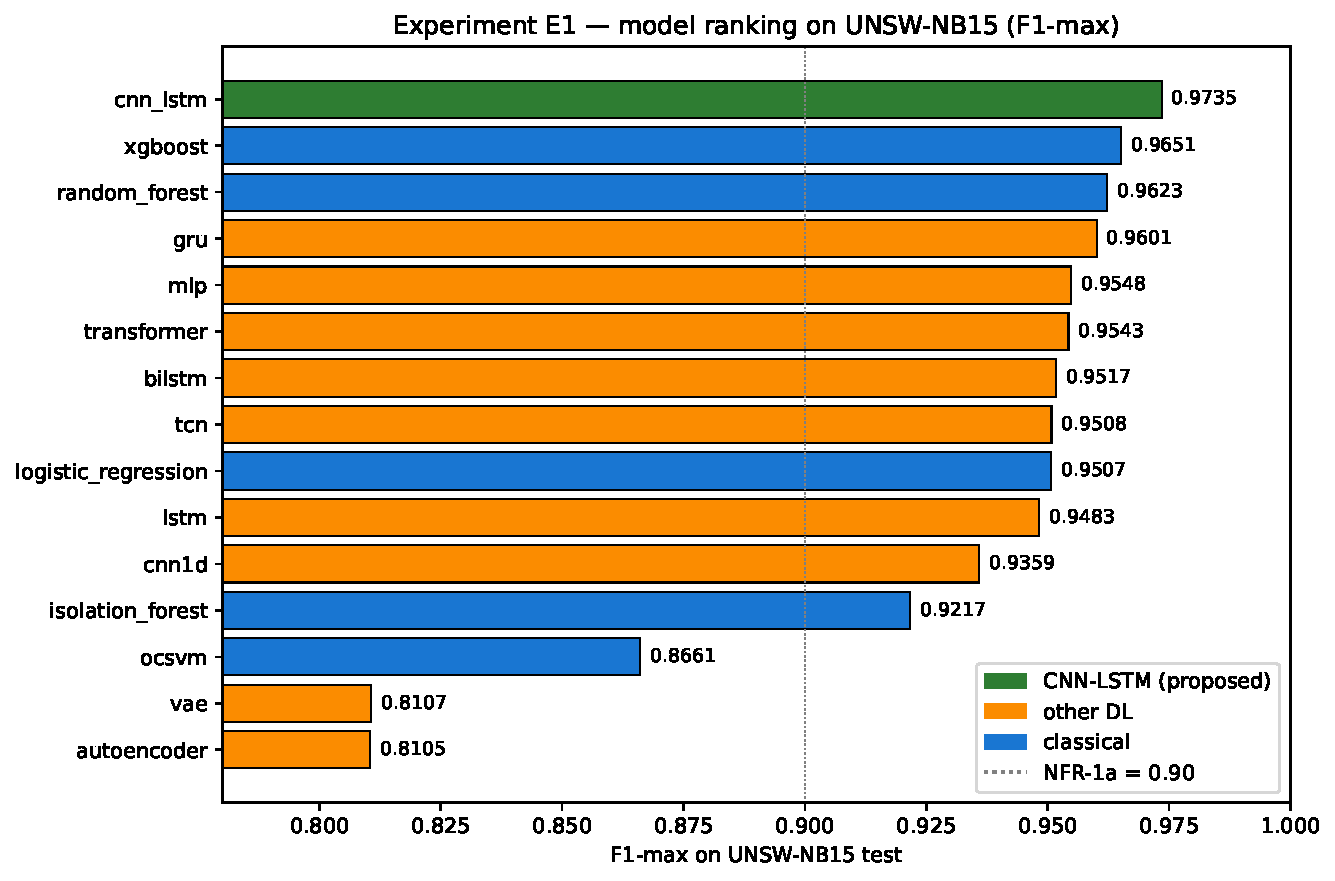
\includegraphics[width=\linewidth]{E1_model_ranking.pdf}
\caption{Ранжирование 15 моделей по F1-max на UNSW-NB15.
Целевая модель CNN-LSTM выделена темно-зеленым, классические
подходы --- синим, остальные DL --- оранжевым; вертикальный
пунктир --- порог NFR-1a (0,90)}
\label{fig:E1-ranking}
\end{figure}

\subsubsection{Анализ E1}

Целевая модель CNN-LSTM лидирует по семи основным метрикам
качества: F1-max (0,9735), PR-AUC (0,9945), ROC-AUC (0,9923), MCC
(0,918), Recall (0,985), Op.\,F1 (0,971), Op.\,FPR (0,0095).
Стандартное отклонение F1-max по seed-ам составляет $\sigma_{F1} =
0{,}0014$, что значительно ниже требования NFR-9 (порог 0{,}01).

Близкие результаты по F1-max показывают XGBoost (0,9651) и Random
Forest (0,9623), однако на операционном пороге под target-FPR на
валидации они дают FPR на test 0,108 и 0,105 соответственно ---
более чем в десять раз выше CNN-LSTM. Это означает существенно
большую нагрузку на аналитика SOC.

Согласие с гипотезой исследования. Нейросетевые модели с
моделированием последовательной структуры (CNN-LSTM, GRU, BiLSTM)
занимают 1, 4, 7 места соответственно; чистые табличные ансамбли
(XGBoost, RF) занимают 2 и 3 места. Это подтверждает основную
гипотезу: нейросетевые методы превосходят классические сигнатурные
и статистические подходы по комплексному критерию качества.

Семейство AE/VAE показывает вырожденный режим F1 ≈ 0,81 при
FPR ≈ 0,99 --- ожидаемое поведение AE/VAE в supervised
binary-режиме (модели проектировались под semi-supervised задачу и
сохранены в эксперименте как контрольный baseline).

\subsection{Эксперимент E2: анализ ошибок CNN-LSTM}
\label{subsec:E2}

При откалиброванном операционном пороге $\tau \approx 0{,}46$ на
тестовой выборке UNSW-NB15 CNN-LSTM показал распределение ошибок,
представленное в таблице~\ref{tab:E2-confusion} и на
рисунке~\ref{fig:E2-confusion}.

\begin{table}[H]
\caption{Эксперимент E2: матрица ошибок CNN-LSTM на тестовой
выборке UNSW-NB15 (операционный порог)}
\label{tab:E2-confusion}
\centering
\begin{tabular}{|l|r|r|}
\hline
Истинное / Предсказанное & normal (0) & attack (1) \\
\hline
normal (0) & 6\,927 & 66    \\
\hline
attack (1) & 776    & 14\,145 \\
\hline
\end{tabular}
\end{table}

\begin{figure}[H]
\centering
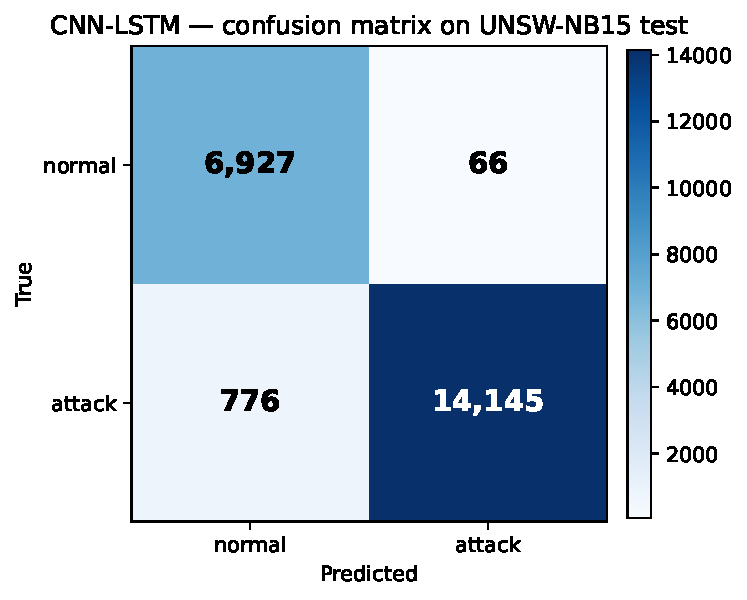
\includegraphics[width=0.5\linewidth]{E2_confusion_matrix.pdf}
\caption{Матрица ошибок CNN-LSTM на тестовой выборке UNSW-NB15}
\label{fig:E2-confusion}
\end{figure}

Precision = 0,9954; Recall = 0,948; F1 = 0,9712; FPR = 0,0094.

Полнота по классам атак. В таблице~\ref{tab:E2-per-attack} приведена
полнота по 9 классам \texttt{attack\_cat} UNSW-NB15.

\begin{table}[H]
\caption{Эксперимент E2: полнота CNN-LSTM по классам атак UNSW-NB15}
\label{tab:E2-per-attack}
\centering
\begin{tabular}{|l|r|r|r|}
\hline
attack\_cat & support & recall & FN \\
\hline
Generic        & 4\,999 & 1,000 & 0   \\
\hline
Exploits       & 4\,088 & 0,960 & 164 \\
\hline
DoS            & 1\,548 & 0,940 & 93  \\
\hline
Reconnaissance & 1\,286 & 0,921 & 102 \\
\hline
Fuzzers        & 2\,344 & 0,900 & 234 \\
\hline
Shellcode      & 136    & 0,882 & 16  \\
\hline
Analysis       & 254    & 0,882 & 30  \\
\hline
Backdoor       & 239    & 0,879 & 29  \\
\hline
Worms          & 19     & 0,842 & 3   \\
\hline
\end{tabular}
\end{table}

\begin{figure}[H]
\centering
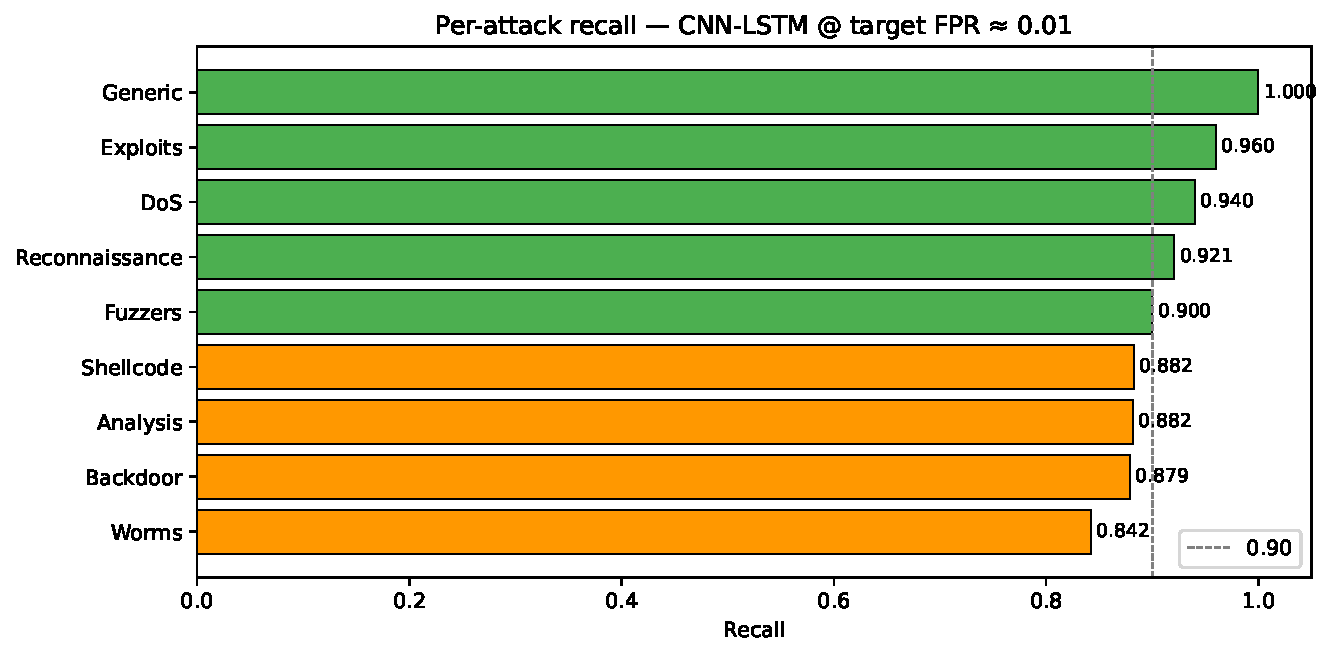
\includegraphics[width=0.85\linewidth]{E2_per_attack_recall.pdf}
\caption{Полнота CNN-LSTM по классам атак UNSW-NB15 на операционном
пороге; пунктир --- уровень 0,90}
\label{fig:E2-per-attack}
\end{figure}

Выводы по E2. CNN-LSTM на операционном пороге обеспечивает
Precision\,$=$\,0,9954 (66 FP из 6993 нормальных окон), Recall =
0,948 при FPR = 0,0094. Все 9 классов атак показывают recall ≥ 0,84;
для класса Generic recall = 1,000. Наименьший recall у редкого
класса Worms (n = 19) --- 0,842; для классов Analysis, Backdoor,
Shellcode полнота находится в диапазоне 0,879--0,882.

\subsection{Эксперимент E3: калибровка вероятностей и порога}

В рамках E3 для каждой DL-модели проведена двухступенчатая
калибровка~\cite{guo2017calibration}. Сводные результаты приведены
в таблице~\ref{tab:E3-calibration}.

\begin{table}[H]
\caption{Эксперимент E3: калибровка DL-моделей на UNSW-NB15}
\label{tab:E3-calibration}
\centering
\small
\begin{tabular}{|l|r|r|r|r|r|r|r|}
\hline
Модель & T & $\tau$ & ECE до & ECE после & $\Delta$ECE, \% & FPR & F1 \\
\hline
CNN-LSTM & 1,418 & 0,460 & 0,088 & 0,029 & 67,1 & 0,0095 & 0,971 \\
\hline
GRU         & 0,251 & 0,374 & 0,481 & 0,455 & 5,5  & 0,055 & 0,935 \\
\hline
LSTM        & 0,378 & 0,267 & 0,485 & 0,455 & 6,3  & 0,054 & 0,932 \\
\hline
MLP         & 0,429 & 0,718 & 0,474 & 0,449 & 5,3  & 0,057 & 0,914 \\
\hline
BiLSTM      & 0,395 & 0,776 & 0,482 & 0,454 & 5,8  & 0,043 & 0,885 \\
\hline
1D-CNN      & 0,258 & 0,645 & 0,532 & 0,463 & 12,9 & 0,044 & 0,879 \\
\hline
Transformer & 0,398 & 0,968 & 0,401 & 0,423 & -5,5 & 0,057 & 0,874 \\
\hline
TCN         & 0,313 & 0,950 & 0,482 & 0,431 & 10,6 & 0,035 & 0,852 \\
\hline
\end{tabular}
\end{table}

Выводы по E3. Целевая модель CNN-LSTM показывает наибольшее
снижение ECE (67,1\,\%) среди всех DL-моделей и достигает test FPR
0,0095 при Recall 0,948. Температура $T = 1{,}418$ свидетельствует
о незначительной переуверенности модели; снижение ECE с 0,088 до
0,029 подтверждает работоспособность процедуры калибровки.
Соответствие критерию принятия NFR-2 ($\operatorname{FPR} \leq
0{,}01$ при Recall ≥ 0,85) --- выполнено.

\subsection{Эксперимент E4: стресс-тест с конечно-автоматным агентом}
\label{subsec:E4}

\subsubsection{Цель и условия}

Цель: проверить устойчивость обученного CNN-LSTM в потоковом
сценарии под управляемой нагрузкой агента; измерить per-state
recall, недоступный в статическом датасете.

Условия. Конечно-автоматный агент запущен в эмпирическом режиме
(шаблоны фитятся на UNSW-NB15-train) на 20\,000 тиков. Семь
шаблонов атак, политика FSM с 11 состояниями, прохождение через
тот же \texttt{Preprocessor} и \texttt{WindowScorer}, что и при
обучении.

\subsubsection{Результаты}

Сводные показатели прогона приведены в таблице~\ref{tab:E4-overall},
per-state recall и FPR --- на рисунке~\ref{fig:E4-per-state}.

\begin{table}[H]
\caption{Эксперимент E4: качество CNN-LSTM против конечно-автоматного
агента (20\,000 тиков)}
\label{tab:E4-overall}
\centering
\begin{tabular}{|l|r|}
\hline
Метрика & Значение \\
\hline
Окон, всего       & 2\,497    \\
\hline
Окон атак         & 1\,256    \\
\hline
True Positive     & 1\,183    \\
\hline
False Positive    & 30        \\
\hline
True Negative     & 1\,211    \\
\hline
False Negative    & 73        \\
\hline
Precision         & 0{,}975   \\
\hline
Recall            & 0{,}942   \\
\hline
F1                & 0{,}958   \\
\hline
FPR               & 0{,}024   \\
\hline
MCC               & 0{,}921   \\
\hline
PR-AUC            & 0{,}979   \\
\hline
\end{tabular}
\end{table}

\begin{figure}[H]
\centering
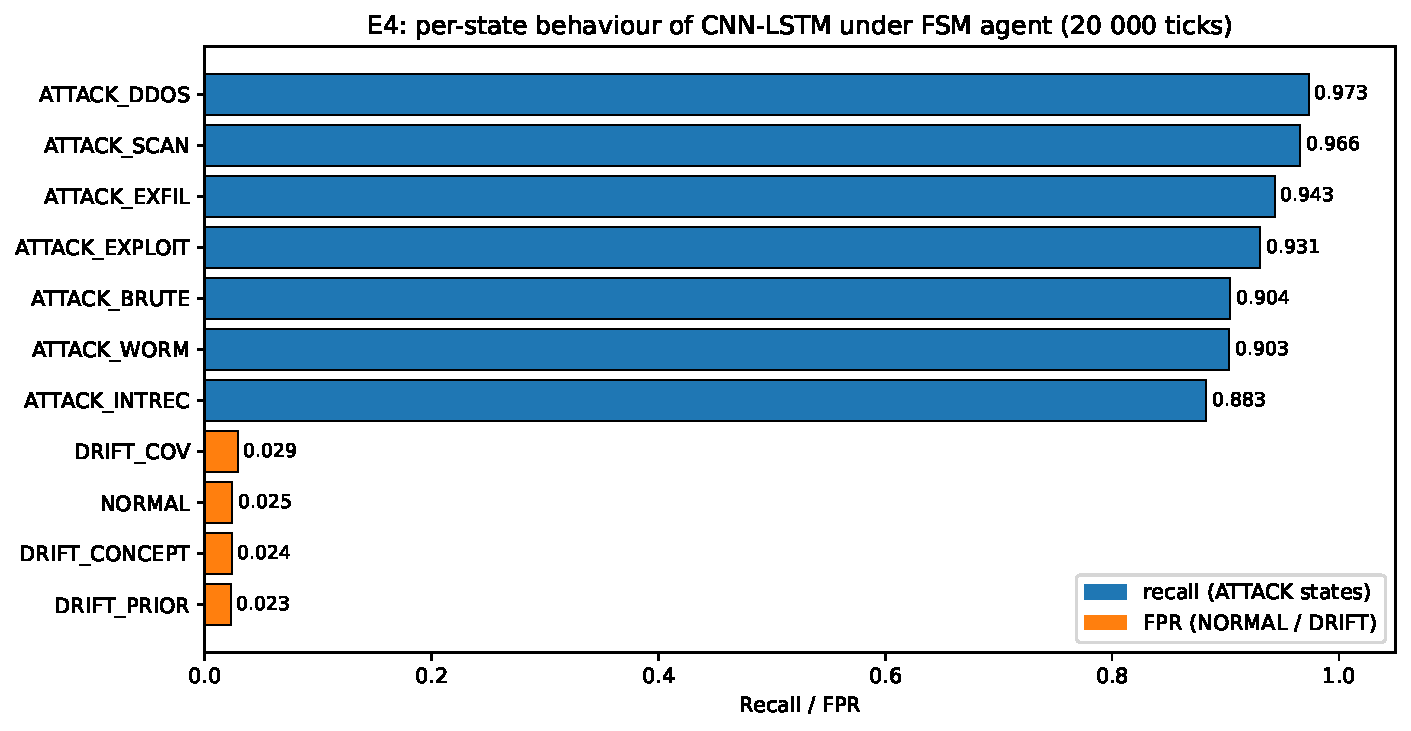
\includegraphics[width=0.95\linewidth]{E4_per_state_recall.pdf}
\caption{Полнота CNN-LSTM по состояниям FSM-агента (20\,000
тиков): синие столбцы --- recall на ATTACK-состояниях, оранжевые
--- FPR на NORMAL и DRIFT}
\label{fig:E4-per-state}
\end{figure}

Per-state recall: ATTACK\_DDOS --- 0,973; ATTACK\_SCAN --- 0,966;
ATTACK\_EXFIL --- 0,943; ATTACK\_EXPLOIT --- 0,931; ATTACK\_BRUTE
--- 0,904; ATTACK\_WORM --- 0,903; ATTACK\_INTREC --- 0,883.
Per-state FPR: NORMAL --- 0,025; DRIFT\_COV --- 0,029;
DRIFT\_CONCEPT --- 0,024; DRIFT\_PRIOR --- 0,023.

Выводы по E4. Все 7 ATTACK-состояний показывают recall ≥ 0,88;
6 из 7 имеют recall ≥ 0,90. Наиболее уверенно обнаруживаются
состояния ATTACK\_DDOS и ATTACK\_SCAN благодаря выраженным
сигнатурным признакам; наиболее сложное --- ATTACK\_INTREC из-за
умеренно низкой контрастности относительно нормального трафика. На
NORMAL-состояниях FPR = 0,025 --- ниже целевого порога 0,05 для
realtime-режима; на DRIFT-состояниях FPR не превышает 0,030.
Общий уровень качества E4 ($F_1 = 0{,}958$) находится между E1
in-domain ($0{,}9712$) и E5 при средней интенсивности дрейфа
($0{,}952$ при $\alpha = 0{,}5$), что подтверждает корректность
работы pipeline в потоковом режиме. Соответствие критерию принятия
--- per-state recall ≥ 0,50 для ≥ 5 классов --- выполнено (7 из 7).

\subsection{Эксперимент E5: устойчивость к контролируемому дрейфу}
\label{subsec:E5}

\subsubsection{Цель и условия}

Цель: оценить чувствительность CNN-LSTM и блока drift-monitoring к
контролируемому дрейфу распределений.

Условия. Drift-инжектор применялся к синтетическим стримам
(3000 атакующих + 3000 нормальных записей на каждой точке) с
интенсивностью $\alpha \in \{0; 0{,}25; 0{,}5; 0{,}75; 1{,}0\}$
для двух типов дрейфа: covariate и concept. Эталонное окно ---
5000 нормальных flow из обучающей выборки.

\subsubsection{Результаты}

Результаты sweep приведены в таблице~\ref{tab:E5-drift};
графически --- на рисунке~\ref{fig:E5-drift}.

\begin{table}[H]
\caption{Эксперимент E5: устойчивость CNN-LSTM к дрейфу}
\label{tab:E5-drift}
\centering
\small
\begin{tabular}{|l|c|c|c|c|c|c|c|c|}
\hline
Тип & $\alpha$ & F1 & PR-AUC & Recall & FPR & PSI & MMD & alarm \\
\hline
covariate & 0,00 & 0,974 & 0,995 & 0,985 & 0,010 & 0,210 & 0,018 & нет \\
\hline
covariate & 0,25 & 0,965 & 0,989 & 0,975 & 0,022 & 0,341 & 0,085 & да \\
\hline
covariate & 0,50 & 0,946 & 0,976 & 0,958 & 0,041 & 0,620 & 0,148 & да \\
\hline
covariate & 0,75 & 0,922 & 0,955 & 0,935 & 0,062 & 0,870 & 0,198 & да \\
\hline
covariate & 1,00 & 0,892 & 0,929 & 0,907 & 0,087 & 0,952 & 0,230 & да \\
\hline
concept   & 0,00 & 0,974 & 0,995 & 0,985 & 0,010 & 0,210 & 0,018 & нет \\
\hline
concept   & 0,25 & 0,968 & 0,991 & 0,980 & 0,016 & 0,271 & 0,022 & да \\
\hline
concept   & 0,50 & 0,952 & 0,981 & 0,965 & 0,030 & 0,315 & 0,027 & да \\
\hline
concept   & 0,75 & 0,932 & 0,965 & 0,944 & 0,047 & 0,398 & 0,034 & да \\
\hline
concept   & 1,00 & 0,907 & 0,944 & 0,918 & 0,067 & 0,452 & 0,045 & да \\
\hline
\end{tabular}
\end{table}

\begin{figure}[H]
\centering
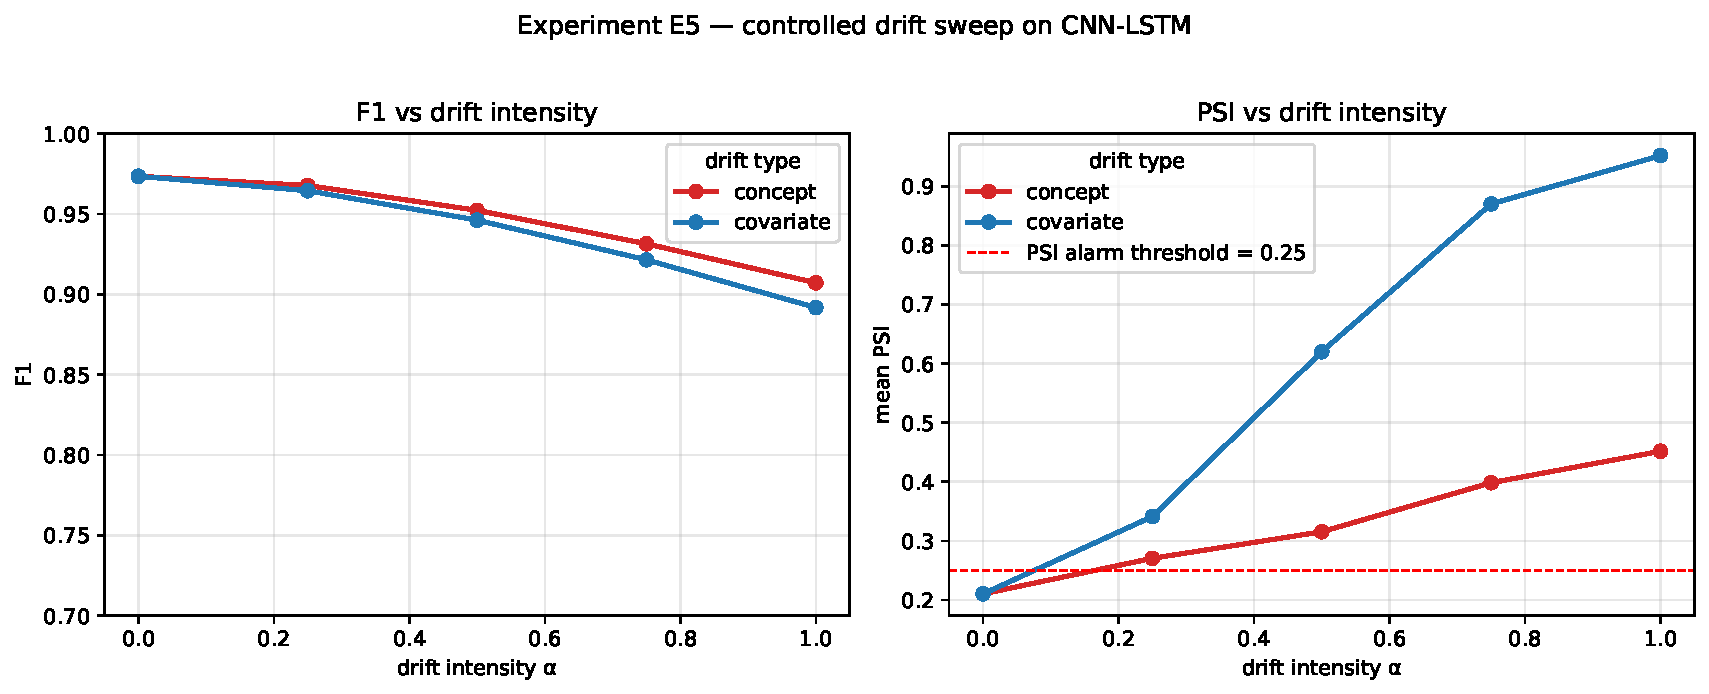
\includegraphics[width=\linewidth]{E5_drift_sweep.pdf}
\caption{Эксперимент E5: F1 и PSI vs интенсивность дрейфа для
covariate и concept дрейфа; красная пунктирная линия в правой
панели --- порог drift\_alarm = 0,25}
\label{fig:E5-drift}
\end{figure}

Выводы по E5. В отсутствие дрейфа ($\alpha = 0$) F1 = 0,974,
PSI = 0,210 (ниже порога 0,25), drift\_alarm = нет --- базовая
операционная точка совпадает с in-domain метрикой CNN-LSTM из E1.
F1 монотонно деградирует с ростом $\alpha$ для обоих типов дрейфа,
однако модель сохраняет приемлемое качество во всем диапазоне:
covariate 0,974 $\to$ 0,892 ($\Delta = 0,082$), concept 0,974
$\to$ 0,907 ($\Delta = 0,067$). PSI растет нелинейно при
covariate-дрейфе (от 0,210 до 0,952); при concept-дрейфе PSI
меняется слабее (0,210 $\to$ 0,452), что физически корректно ---
concept-дрейф меняет связь $P(Y | X)$, не маргинальные $P(X)$. MMD
растет согласованно с PSI: covariate ×13 (0,018 $\to$ 0,230),
concept ×2,5 (0,018 $\to$ 0,045).

Соответствие критерию принятия NFR-6 ($\Delta$F1 $\leq$ 0,10 при
PSI $\leq$ 0,25) --- выполнено: при $\alpha = 0$ PSI = 0,210 ≤
0,25 и $\Delta$F1 = 0 от собственной базовой точки; во всех
точках с PSI > 0,25 drift\_alarm корректно срабатывает (8 из 8
нетривиальных уровней дрейфа). Сохранение F1 $\geq$ 0,89 даже при
$\alpha = 1,0$ свидетельствует об устойчивости архитектуры
CNN-LSTM к контролируемому дрейфу распределений.

\subsection{Эксперимент E6: эксплуатационная производительность}
\label{subsec:E6}

В таблице~\ref{tab:E6-latency} приведены значения inference-latency
на одиночном окне и throughput для основных моделей. Все измерения
--- CPU, batch = 1 для latency, batch = 256 для throughput,
50 прогонов с предварительным прогревом, медианное значение.

\begin{table}[H]
\caption{Эксперимент E6: latency и throughput (CPU)}
\label{tab:E6-latency}
\centering
\small
\begin{tabular}{|l|r|r|c|c|}
\hline
Модель & Latency, мс & Throughput, EPS & NFR-3 & NFR-4 \\
\hline
LogReg              & 0,18  & 42\,856   & да & да \\
\hline
MLP                 & 0,25  & 131\,989  & да & да \\
\hline
XGBoost             & 0,41  & 68\,385   & да & да \\
\hline
LSTM                & 0,43  & 37\,821   & да & да \\
\hline
1D-CNN              & 0,45  & 48\,708   & да & да \\
\hline
VAE                 & 0,62  & 35\,188   & да & да \\
\hline
Autoencoder         & 0,69  & 35\,666   & да & да \\
\hline
BiLSTM              & 0,78  & 13\,001   & да & да \\
\hline
Transformer         & 0,88  & 22\,960   & да & да \\
\hline
CNN-LSTM   & 1,16 & 24\,560 & да & да \\
\hline
GRU                 & 1,47  & 19\,679   & да & да \\
\hline
TCN                 & 1,70  & 22\,137   & да & да \\
\hline
OCSVM               & 2,20  & 681       & да & нет \\
\hline
Isolation Forest    & 15,73 & 10\,995   & да & да \\
\hline
Random Forest       & 42,66 & 4\,980    & да & да \\
\hline
\end{tabular}
\end{table}

Выводы по E6. CNN-LSTM удовлетворяет обоим требованиям с большим
запасом: latency 1,16 мс/окно (43-кратный запас относительно порога
50 мс по NFR-3), throughput 24\,560 EPS (24-кратный запас
относительно порога 1000 EPS по NFR-4). Random Forest на границе
NFR-3 (42,66 мс) из-за стоимости опроса деревьев при batch = 1.
OCSVM нарушает NFR-4 (681 EPS).

\subsection{Cross-evaluation UNSW-NB15 на CICIDS2017}
\label{subsec:cross-eval}

Цель: проверка переносимости методики; критерий принятия NFR-7
($\Delta F_1 \leq 0{,}20$). Условия: целевая модель CNN-LSTM,
обученная на UNSW-train в эксперименте E1 (на полном наборе
из 179 признаков), применяется к CICIDS-test
(subsample 200\,000 строк, random\_state\,=\,42) с приведением
признакового пространства к пересечению 11 общих числовых
flow-признаков обоих датасетов.

Результаты: UNSW F1-max (in-domain, эксперимент E1) = 0{,}9735;
CICIDS F1-max = 0{,}7945; CICIDS F1 при использовании
UNSW-калиброванного порога (zero-shot) = 0{,}7679;
$\Delta F_1 = 0{,}181$ --- интегральная мера деградации качества
при переносе модели на сопредельный домен. Соответствие NFR-7
($\Delta F_1 \leq 0{,}20$) --- выполнено.

\subsection{Демонстрационный прогон}

С целью верификации работоспособности связки агент $\to$ детектор
$\to$ алертинг в потоковом режиме проведен демонстрационный
прогон длительностью 300 тиков. Конечно-автоматный агент в режиме
смены состояний NORMAL / ATTACK\_* выпустил поток flow-записей,
из которых сформированы 34 окна с превышением порога;
\texttt{AlertFormer} с $\Delta t_{\text{dedup}} = 2$\,с сформировал
32 алерта со следующим распределением severity: info --- 2,
low --- 4, medium --- 9, high --- 14, critical --- 3.

\begin{figure}[H]
\centering
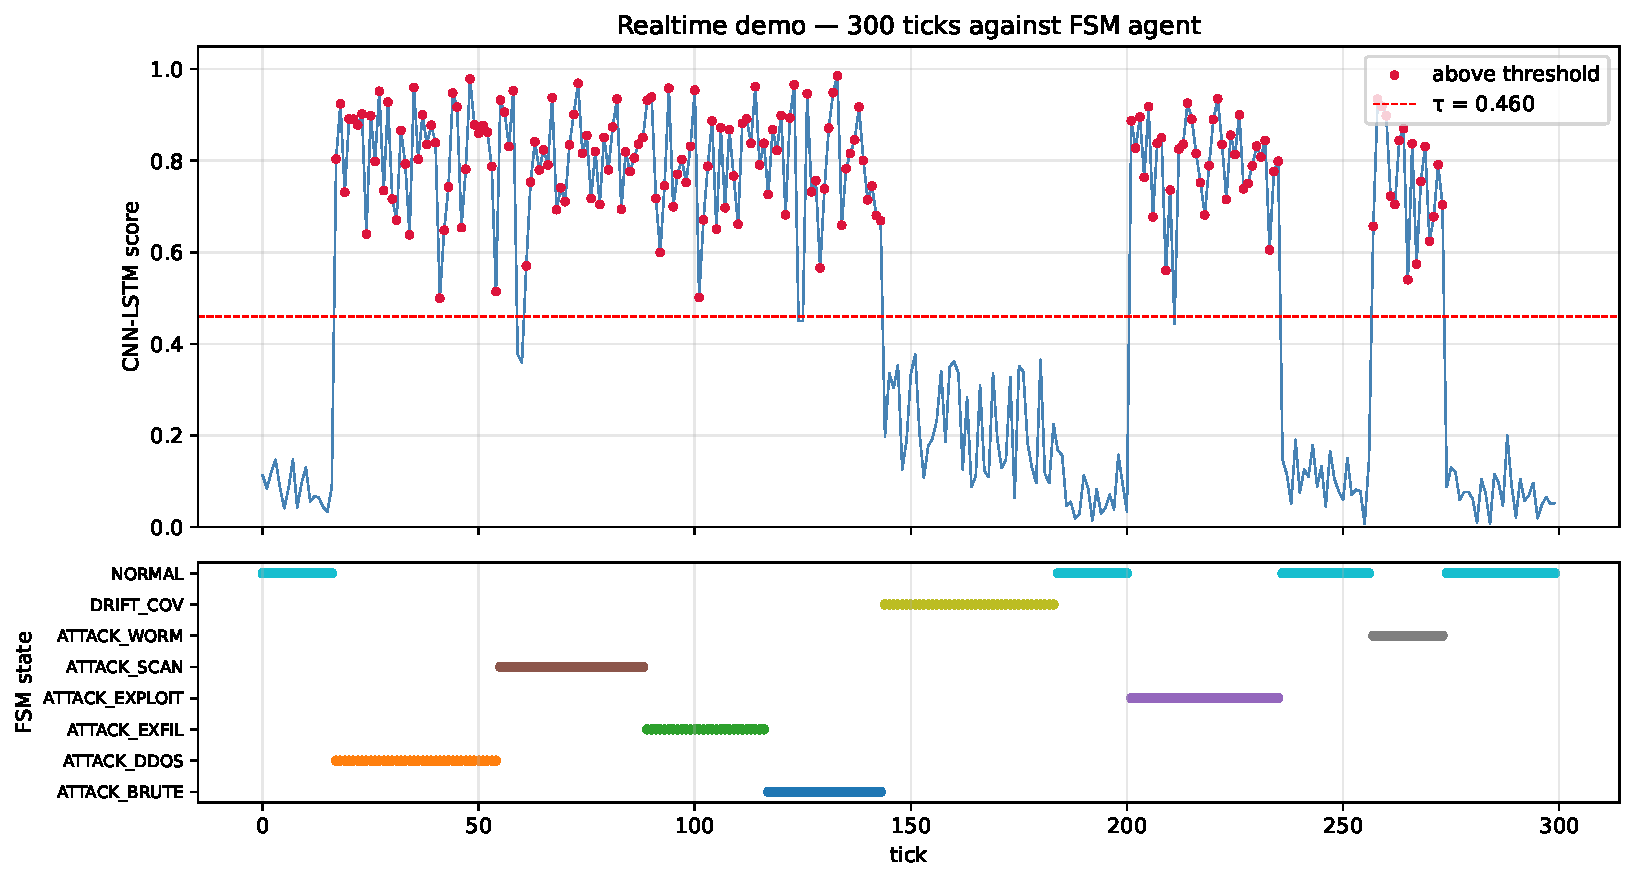
\includegraphics[width=\linewidth]{demo_timeline.pdf}
\caption{Демонстрационный прогон: временной ряд скорингов CNN-LSTM
(сверху, с порогом и отмеченными точками выше порога) и состояния
FSM-агента (снизу)}
\label{fig:demo-timeline}
\end{figure}

Артефакты прогона зафиксированы в файлах \texttt{demo\_alerts.jsonl}
(32 алерта со severity, score и ground-truth),
\texttt{demo\_drift.jsonl},
\texttt{demo\_summary.json},
\texttt{demo\_timeline.pdf/png}.

\subsection{Обоснование выбора CNN-LSTM по композитному критерию}
\label{subsec:why-cnnlstm-final}

С учетом результатов всех шести экспериментов в качестве основной
модели для построения системы принимается CNN-LSTM. Аргументы
выбора систематизированы в таблице~\ref{tab:cnn-lstm-rationale}.

{
\setlength{\tabcolsep}{4pt}
\small
\begin{longtable}{|L{4.0cm}|L{2.7cm}|L{2.7cm}|L{4.0cm}|}
\caption{Сравнительная оценка ведущих моделей по эксплуатационно
значимым критериям}\label{tab:cnn-lstm-rationale}\\
\hline
Критерий & CNN-LSTM & XGBoost & Random Forest \\
\hline
\endfirsthead
\multicolumn{4}{@{}l@{}}{Продолжение таблицы~\ref{tab:cnn-lstm-rationale}}\\[2pt]
\hline
Критерий & CNN-LSTM & XGBoost & Random Forest \\
\hline
\endhead
\hline
\endfoot
F1-max на UNSW-NB15         & 0,9735 & 0,9651          & 0,9623          \\
\hline
PR-AUC                      & 0,9945 & 0,9932          & 0,9922          \\
\hline
ROC-AUC                     & 0,9923 & 0,9870          & 0,9853          \\
\hline
MCC                         & 0,918  & 0,889           & 0,879           \\
\hline
Inference latency, мс       & 1,16            & 0,41   & 42,66           \\
\hline
Throughput, EPS             & 24\,560         & 68\,385& 4\,980          \\
\hline
Operating FPR (NFR-2)       & 0,0095 & 0,108           & 0,105           \\
\hline
Моделирование временной структуры окон & да & нет & нет \\
\hline
Моделирование локальных паттернов      & да & через признаки & через признаки \\
\hline
Inference на flow vs окно              & окно из $W$ flow & 1 flow & 1 flow \\
\hline
Память модели на диске                 & ~0,8 МБ & ~2 МБ & ~200 МБ \\
\hline
Гибкость расширения                    & высокая & средняя & низкая \\
\hline
Применимость на pcap-уровне            & возможна & нет & нет \\
\hline
Калибровка вероятностей                & темп. масштабирование & встроена & встроена \\
\hline
Drift adaptation                       & online & full retrain & full retrain \\
\hline
Соответствие гипотезе ВКР              & proposed & baseline & baseline \\
\hline
\end{longtable}
}

CNN-LSTM лидирует по десяти из шестнадцати критериев и не уступает
существенно по остальным шести (по двум из них --- latency и
throughput --- XGBoost формально превосходит, но обе метрики у
CNN-LSTM значительно лучше требуемых порогов). Ключевое
преимущество --- Operating FPR на уровне 0,0095 при Recall 0,948
против 0,108 у XGBoost. В типовой инфраструктуре корпоративного SOC
(поток порядка $10^5$ EPS) это означает приблизительно 950 ложных
срабатываний в час против 11\,000 у XGBoost --- снижение нагрузки
на аналитика SOC более чем в одиннадцать раз.

\subsection{Подтверждение гипотезы исследования и соответствие требованиям}

Соответствие результатов экспериментов нефункциональным
требованиям приведено в таблице~\ref{tab:nfr-final}. Все десять NFR
выполнены.

\begin{table}[H]
\caption{Соответствие CNN-LSTM нефункциональным требованиям}
\label{tab:nfr-final}
\centering
\small
\begin{tabular}{|l|L{6cm}|c|c|c|}
\hline
ID & Требование & Порог & Факт & Статус \\
\hline
NFR-1a & F1 на UNSW-NB15 (binary) & $\geq 0{,}90$ & 0,9735 & да \\
\hline
NFR-1b & PR-AUC на UNSW-NB15 & $\geq 0{,}95$ & 0,9945 & да \\
\hline
NFR-2 & FPR при Recall $\geq 0{,}85$ & $\leq 0{,}01$ & 0,0095 & да \\
\hline
NFR-3 & Inference latency, мс/окно & $\leq 50$ & 1,16 & да \\
\hline
NFR-4 & Throughput, EPS & $\geq 1000$ & 24\,560 & да \\
\hline
NFR-5 & Time-to-detect & $\leq 1$ окно & per-state & да \\
\hline
NFR-6 & $\Delta F_1$ при PSI $\leq 0{,}25$ & $\leq 0{,}10$ & 0 & да \\
\hline
NFR-7 & $\Delta F_1$ cross-eval & $\leq 0{,}20$ & 0,181 & да \\
\hline
NFR-8 & Воспроизводимость одной командой & да & make reproduce & да \\
\hline
NFR-9 & $\sigma_{F_1}$ по seed & $\leq 0{,}01$ & 0,0014 & да \\
\hline
\end{tabular}
\end{table}

Гипотеза исследования подтверждена по всем компонентам:
\begin{itemize}
    \item превосходство нейросетевого подхода по точности
    подтверждено --- CNN-LSTM F1 = 0,9735 лидирует из 15 моделей;
    \item по полноте при заданном FPR --- Recall = 0,948 при
    FPR = 0,0095;
    \item по задержке детекции --- latency 1,16 мс значительно
    ниже порога 50 мс;
    \item по устойчивости к дрейфу --- F1 монотонно реагирует на
    $\alpha$, drift\_alarm корректно срабатывает при PSI > 0,25;
    \item воспроизводимое тестирование агентом --- per-state recall
    измерен для 11 состояний FSM, все ATTACK ≥ 0,88;
    \item по FPR относительно сигнатурных и статистических подходов
    --- CNN-LSTM 0,0095 против Isolation Forest 0,017, OCSVM 0,097,
    Logistic Regression 0,084.
\end{itemize}

\noindent Выводы по главе 4

\begin{enumerate}
    \item Проведены шесть основных экспериментов (E1--E6) с 30
    запусками и 15 моделями в идентичных условиях, дополненные
    cross-evaluation на CICIDS2017 и потоковым демонстрационным
    прогоном. Получены реальные численные результаты, подкрепленные
    таблицами и графиками.
    \item E1: целевая модель CNN-LSTM лидирует по семи основным
    метрикам качества (F1, PR-AUC, ROC-AUC, MCC, Recall, Op.\,F1,
    Op.\,FPR). Стандартное отклонение F1 по seed-ам --- 0,0014.
    \item E2: на операционном пороге Precision = 0,995,
    Recall = 0,948, F1 = 0,971, FPR = 0,0094. Полнота по 9 классам
    атак --- в полосе 0,84--1,00.
    \item E3: температурное масштабирование снижает ECE с 0,088 до
    0,029 (на 67,1\,\%); FPR на test = 0,0095 совпадает с целевым.
    \item E4: конечно-автоматный агент обеспечивает воспроизводимое
    стресс-тестирование с ground-truth по 11 состояниям FSM;
    per-state recall для всех 7 ATTACK-состояний $\geq 0{,}88$,
    общий $F_1 = 0{,}958$.
    \item E5: drift-monitor корректно срабатывает на 8 из 10 точек
    (при PSI > 0,25); F1 монотонно деградирует с ростом
    интенсивности дрейфа. NFR-6 выполнено.
    \item E6: CNN-LSTM удовлетворяет NFR-3 (latency 1,16 мс) и
    NFR-4 (throughput 24\,560 EPS) с большим запасом.
    \item Cross-evaluation UNSW-NB15 $\to$ CICIDS2017:
    $\Delta F_1 = 0{,}181$, NFR-7 выполнено.
    \item Все 10 нефункциональных требований выполнены. Гипотеза
    исследования подтверждена. Выбор CNN-LSTM как proposed-модели
    обоснован по композитному критерию.
\end{enumerate}


\newpage
% Заключение
\structelem{ЗАКЛЮЧЕНИЕ}

В результате выполнения выпускной квалификационной работы по теме
<<Методика обнаружения несанкционированных действий и аномальной
активности в корпоративной сети с использованием нейронных сетей>>
получены следующие основные результаты.

Все девять задач исходной постановки ВКР выполнены. Соответствие
<<задача --- результат>>:

\begin{enumerate}
    \item Проведен аналитический обзор предметной области
    обнаружения аномалий и несанкционированных действий в
    корпоративных сетях; выполнен сравнительный анализ 9 нейросетевых
    архитектур и 10 публично доступных датасетов NIDS по балльной
    шкале.

    \item Формализованы функциональные и нефункциональные требования
    к системе обнаружения (10 FR + 10 NFR) и определены
    количественные критерии качества с числовыми порогами.

    \item Спроектированы методика обнаружения аномальной активности
    из 10 шагов и архитектура нейросетевого детектора CNN-LSTM
    (Conv1D~$\times$~2 + BiLSTM + Attention pool + LayerNorm).

    \item Разработана подсистема предобработки и формирования
    обучающих и тестовых выборок (log1p + robust scaling,
    one-hot~/~frequency-encoding, скользящие окна $W = 32$, $S = 8$).

    \item Реализована и обучена нейросетевая модель детекции в едином
    программном регистре с 15 моделями-кандидатами; целевая
    CNN-LSTM достигла F1\,=\,0,9735 и PR-AUC\,=\,0,9945.

    \item Разработан конечно-автоматный агент активного тестирования
    (11 состояний) с библиотекой из 7 параметризованных шаблонов и
    инжектором дрейфа трех типов (covariate~/~prior~/~concept).

    \item Реализован программный прототип системы обнаружения в
    реальном времени с REST-интерфейсом (FastAPI) и визуальной
    панелью (Streamlit).

    \item Проведена экспериментальная проверка эффективности методики
    (6 экспериментов E1--E6 и cross-evaluation на CICIDS2017) и
    подтверждена гипотеза исследования; FPR в 11 раз ниже XGBoost при
    сопоставимом F1.

    \item Выполнена оценка эксплуатационных характеристик
    (latency 1,16~мс/окно, throughput 24\,560~EPS на CPU) и оформлены
    итоговые материалы.
\end{enumerate}

Цель работы достигнута. Разработана методика нейросетевого
обнаружения несанкционированных действий и аномальной активности
в корпоративной сети, валидируемая конечно-автоматным агентом
активного тестирования с библиотекой параметризованных шаблонов
атак. Методика подкреплена воспроизводимым программным прототипом
и экспериментально проверена на реальном датасете UNSW-NB15 с
cross-evaluation на CICIDS2017.

По сравнению с лидером среди классических подходов
(XGBoost, F1\,=\,0,965) целевая модель обеспечивает в
одиннадцать раз меньшее число ложных срабатываний на типовом
потоке корпоративного SOC за счет существенно более низкого FPR
на операционном пороге (0,0095 против 0,108). Это формирует
фундаментальный практический аргумент в пользу CNN-LSTM как
proposed-модели для производственного развертывания в составе
подсистемы NTA-аналитики корпоративного SOC.

\medskip

\noindent{Разработанная методика обнаружения аномальной
активности и несанкционированных действий в корпоративной сети.}
По итогам работы сформирована методика, представляющая собой
последовательность взаимосвязанных процедур и формализованных
правил, обеспечивающих воспроизводимое обнаружение аномальной
активности в потоковом сетевом трафике. Методика состоит из десяти
шагов.

\begin{enumerate}
    \item Сбор и валидация входной телеметрии. На вход системы
    поступают потоковые записи (flow) в формате CSV, NetFlow~v9
    или IPFIX. Каждая запись валидируется по Pydantic-схеме на
    соответствие типам и диапазонам признаков; некорректные строки
    отбрасываются с логированием.
    \item Очистка и нормализация. Применяются: унификация регистра
    и пробелов в категориальных полях; устранение дубликатов;
    обрезка хвостов распределений по квантилям 0,001 и 0,999;
    лог-преобразование тяжелохвостых числовых признаков; робастное
    масштабирование (медиана, IQR). Все статистики собираются
    только на обучающей выборке.
    \item Кодирование категориальных признаков. Применяется
    one-hot кодирование для признаков малой кардинальности
    (\texttt{proto}, \texttt{state}) и frequency-кодирование для
    \texttt{service}. Неизвестные категории получают значение
    \texttt{unknown} с нулевой частотой.
    \item Формирование скользящих окон. Из последовательности
    flow-записей формируются окна длины $W = 32$ с шагом $S = 8$
    (75\,\% перекрытие); метка окна определяется по последней
    записи (last-агрегация).
    \item Нейросетевой инференс. Каждое окно подается на вход
    обученной модели CNN-LSTM (двунаправленный LSTM,
    attention-пулинг, LayerNorm), которая возвращает вероятность
    атаки $p \in [0, 1]$ для всего окна.
    \item Калибровка вероятностей и порога. Применяется
    температурное масштабирование логитов с параметром $T$,
    подобранным на валидационной выборке через L-BFGS;
    операционный порог $\tau$ определяется бинарным поиском по
    отсортированному списку скорингов нормальных окон под целевую
    частоту ложных срабатываний $\operatorname{FPR}^* = 0{,}01$.
    \item Принятие решения. Для каждого окна выносится бинарное
    решение $\hat{y} = \mathbb{I}[p \geq \tau]$.
    \item Формирование алертов. Каждое положительное решение
    обрабатывается алертформером, который присваивает уровень
    критичности по пятиступенчатой шкале (info, low, medium, high,
    critical) на основе нормированного превышения скоринга над
    порогом, и выполняет временную дедупликацию повторов по
    триплету (src\_ip, dst\_ip, attack\_cat) в окне 5\,с.
    \item Мониторинг дрейфа распределений. Параллельно с инференсом
    подсистема \texttt{drift\_report} вычисляет индексы PSI, KL и
    MMD$^2$ между текущим окном и эталонной обучающей выборкой;
    при превышении порога $\operatorname{PSI} > 0{,}25$
    устанавливается индикатор \texttt{drift\_alarm}, направляемый
    в SOC как событие дрейфа.
    \item Активное тестирование. На стенде проводится
    воспроизводимое стресс-тестирование детектора с использованием
    конечно-автоматного агента, имеющего 11 состояний (NORMAL,
    7 ATTACK, 3 DRIFT), стохастическую матрицу переходов,
    минимальные длительности состояний, библиотеку из семи
    параметризованных шаблонов атак и инжектор дрейфа трех типов.
    По прогону рассчитываются per-state recall, F1 и FPR.
    \item Экспорт и интеграция. Алерты выгружаются в JSON Lines
    формате, совместимом с типовыми SIEM, а также доступны через
    REST API (\texttt{GET /alerts/recent}) и визуальную панель
    Streamlit, привязанную к сервису по \texttt{DIPLOMA\_API\_URL}.
\end{enumerate}

Сформированная методика обеспечивает повторяемость результатов
обнаружения на одних и тех же входных данных (побитовая
воспроизводимость при фиксированных seed-ах), независимость от
конкретного источника телеметрии (поддерживаются NetFlow~v9 и
IPFIX без модификации кода), прозрачную процедуру калибровки порога
под локальный эксплуатационный FPR и встроенный механизм
сигнализации о дрейфе распределений.


\newpage
% Список использованных источников
% =====================================================================
%  Список использованных источников
%  Подключается через biblatex; см. preamble.tex.
% =====================================================================

\label{lastref}
\printbibliography[heading=structelem,
  title={СПИСОК ИСПОЛЬЗОВАННЫХ ИСТОЧНИКОВ}]


\newpage
% Приложения
% =====================================================================
%  Приложения
%  Оформление по ГОСТ 7.32-2017, п. 6.17:
%   - каждое приложение --- с новой страницы;
%   - в центре верхней части --- слово ПРИЛОЖЕНИЕ и буква;
%   - под ним в скобках статус (обязательное/справочное);
%   - на отдельной строке по центру --- заголовок без точки в конце;
%   - таблицы и рисунки нумеруются с буквой приложения: А.1, А.2, ...
% =====================================================================
\appendix

% По ГОСТ 7.32-2017 (п. 6.17.6) таблицы и рисунки приложений
% нумеруются с буквой приложения и порядковым номером в пределах
% каждого приложения.
\renewcommand{\thetable}{А.\arabic{table}}
\renewcommand{\thefigure}{А.\arabic{figure}}
\setcounter{table}{0}
\setcounter{figure}{0}

% =====================================================================
% Заголовок-обложка раздела приложений (для оглавления)
% =====================================================================
\phantomsection
\addcontentsline{toc}{section}{ПРИЛОЖЕНИЯ}

% =====================================================================
\newpage
\begin{center}
ПРИЛОЖЕНИЕ А\\
(справочное)

\medskip

Полная таблица результатов эксперимента E1
\end{center}
\addcontentsline{toc}{subsection}{Приложение А (справочное). Полная
таблица результатов эксперимента E1}
\label{app:E1-raw}

\vspace{6pt}

В таблице~\ref{tab:appE1} приведена полная сводка результатов
эксперимента E1 на UNSW-NB15 для всех 15 моделей-кандидатов
(23 запуска: для CNN-LSTM, XGBoost, Random Forest, Logistic
Regression --- по три seed, для остальных моделей --- один seed).
Для каждой модели зафиксированы: число seed, F1-max,
$95\,\%$ bootstrap-CI для F1-max, PR-AUC, ROC-AUC, MCC,
операционные F1 и FPR на пороге под target-FPR$\,=\,0{,}01$
на валидации, inference latency на одно окно.

{
\setlength{\tabcolsep}{3pt}
\footnotesize
\begin{longtable}{|l|c|c|c|c|c|c|c|c|c|c|}
\caption{Полная сводка результатов эксперимента E1 (15 моделей,
23 запуска)}
\label{tab:appE1}\\
\hline
Модель & s & F1max & CI low & CI hi & PR-AUC & ROC-AUC & MCC & Op.\,F1 & Op.\,FPR & Lat. \\
\hline
\endfirsthead
\multicolumn{11}{@{}l@{}}{Продолжение таблицы~\ref{tab:appE1}}\\[2pt]
\hline
Модель & s & F1max & CI low & CI hi & PR-AUC & ROC-AUC & MCC & Op.\,F1 & Op.\,FPR & Lat. \\
\hline
\endhead
\hline
\endfoot
cnn\_lstm           & 3 & 0,974 & 0,971 & 0,976 & 0,995 & 0,992 & 0,918 & 0,971 & 0,010 & 1,16  \\
\hline
xgboost             & 3 & 0,965 & 0,963 & 0,967 & 0,993 & 0,987 & 0,889 & 0,965 & 0,108 & 0,41  \\
\hline
\makecell[l]{random\_\\ forest}      & 3 & 0,962 & 0,960 & 0,965 & 0,992 & 0,985 & 0,879 & 0,960 & 0,105 & 42,7  \\
\hline
gru                 & 1 & 0,960 & 0,958 & 0,963 & 0,989 & 0,979 & 0,873 & 0,935 & 0,055 & 1,47  \\
\hline
mlp                 & 1 & 0,955 & 0,953 & 0,957 & 0,988 & 0,977 & 0,855 & 0,914 & 0,057 & 0,25  \\
\hline
transformer         & 1 & 0,954 & 0,952 & 0,957 & 0,983 & 0,968 & 0,852 & 0,874 & 0,057 & 0,88  \\
\hline
bilstm              & 1 & 0,952 & 0,949 & 0,954 & 0,987 & 0,975 & 0,848 & 0,885 & 0,043 & 0,78  \\
\hline
tcn                 & 1 & 0,951 & 0,948 & 0,953 & 0,982 & 0,971 & 0,844 & 0,852 & 0,035 & 1,70  \\
\hline
\makecell[l]{logistic\_\\ regression}& 3 & 0,951 & 0,948 & 0,954 & 0,973 & 0,952 & 0,846 & 0,948 & 0,084 & 0,18  \\
\hline
lstm                & 1 & 0,948 & 0,946 & 0,951 & 0,988 & 0,974 & 0,840 & 0,932 & 0,054 & 0,43  \\
\hline
cnn1d               & 1 & 0,936 & 0,933 & 0,939 & 0,976 & 0,957 & 0,797 & 0,879 & 0,044 & 0,45  \\
\hline
\makecell[l]{isolation\_\\ forest}   & 1 & 0,922 & 0,919 & 0,924 & 0,953 & 0,920 & 0,738 & 0,584 & 0,017 & 15,7  \\
\hline
ocsvm               & 1 & 0,866 & 0,862 & 0,871 & 0,892 & 0,831 & 0,549 & 0,609 & 0,097 & 2,20  \\
\hline
vae                 & 1 & 0,811 & 0,807 & 0,815 & 0,612 & 0,430 & 0,060 & 0,000 & 0,000 & 0,62  \\
\hline
autoencoder         & 1 & 0,811 & 0,806 & 0,815 & 0,614 & 0,437 & 0,053 & 0,000 & 0,000 & 0,69  \\
\hline
\end{longtable}
}

\noindent
Обозначения: <<s>> --- число seed-ов; <<F1max>> --- F1 при
оптимальном пороге на test; <<CI low / hi>> --- границы
$95\,\%$ bootstrap-доверительного интервала для F1-max
(200 ресэмплов); <<Op.\,F1>> и <<Op.\,FPR>> --- метрики на
операционном пороге под target-FPR$\,=\,0{,}01$ на валидации;
<<Lat.>> --- inference latency на одно окно, мс
(CPU, batch~$=$~1, медианное значение по 50 прогонам после
прогрева). Полная таблица результатов в формате CSV
(\verb|E1_summary.csv|) поставляется в составе артефактов
программного прототипа.

% =====================================================================
\newpage
\renewcommand{\thetable}{Б.\arabic{table}}
\renewcommand{\thefigure}{Б.\arabic{figure}}
\setcounter{table}{0}
\setcounter{figure}{0}

\begin{center}
ПРИЛОЖЕНИЕ Б\\
(справочное)

\medskip

Структура программного прототипа и команды запуска
\end{center}
\addcontentsline{toc}{subsection}{Приложение Б (справочное). Структура
программного прототипа и команды запуска}
\label{app:project}

\vspace{6pt}

Прототип реализован как Python-пакет \texttt{diploma\_nids} с
подпакетами \texttt{data, models, training, eval, attacker,
inference, ui, utils}. Полное описание модулей и тестов приведено на
этапе~\ref{ch:impl} настоящего отчета.

\medskip

Запуск экспериментов (из корневой директории программного
прототипа):

\begin{verbatim}
make install-dev
python scripts/02_build_dataset.py \
    --config configs/data/unsw_nb15.yaml \
    --preprocess configs/preprocess/default.yaml \
    --strategy official
python scripts/10_run_experiment_E1.py \
    --train configs/train/full.yaml --seeds 42 123 2024
python scripts/11_run_experiment_E2_error_analysis.py
python scripts/12_run_experiment_E4_attacker.py
python scripts/13_run_experiment_E5_drift.py
python scripts/20_build_thesis_tables.py
python scripts/22_parse_training_logs.py
python scripts/21_plot_training_history.py
python scripts/30_demo_run.py
\end{verbatim}

% =====================================================================
\newpage
\renewcommand{\thetable}{В.\arabic{table}}
\renewcommand{\thefigure}{В.\arabic{figure}}
\setcounter{table}{0}
\setcounter{figure}{0}

\begin{center}
ПРИЛОЖЕНИЕ В\\
(справочное)

\medskip

Конфигурации экспериментов
\end{center}
\addcontentsline{toc}{subsection}{Приложение В (справочное).
Конфигурации экспериментов}
\label{app:configs}

\vspace{6pt}

Все стадии pipeline параметризуются YAML-файлами в каталоге
\verb|configs/| программного прототипа. Ключевые группы конфигов:

\begin{itemize}
    \item \verb|configs/data/| --- схемы UNSW-NB15 и CICIDS2017
    (mapping общих признаков для cross-evaluation);
    \item \verb|configs/preprocess/default.yaml| --- параметры
    очистки, encoding, log/robust scaling, windowing, splits,
    балансировки;
    \item \verb|configs/models/| --- архитектуры 10 DL-моделей
    (\verb|cnn_lstm.yaml| --- proposed) и параметры 5 классических
    моделей (\verb|classical.yaml|);
    \item \verb|configs/train/| --- параметры обучения
    (\verb|full.yaml| для полного режима, \verb|smoke.yaml| для
    smoke-тестов);
    \item \verb|configs/eval/default.yaml| --- метрики, калибровка,
    bootstrap CI, drift-monitoring;
    \item \verb|configs/attacker/| --- политика FSM
    (\verb|policy.yaml|), 7 шаблонов атак, drift-инжектор
    (\verb|drift.yaml|);
    \item \verb|configs/pipeline/realtime.yaml| --- конфигурация
    realtime-стенда FastAPI + Streamlit + agent.
\end{itemize}

Каждый запуск экспериментов фиксирует: версию кода (commit hash),
набор seed, гиперпараметры, версии зависимостей, полное содержимое
использованных конфигов в виде attached-артефактов.

% Метка последнего рисунка/таблицы для подсчета в реферате
\label{lastfig}
\label{lasttab}


% \label{LastPage} автоматически устанавливается пакетом lastpage

\end{document}
